\documentclass[10pt]{beamer}

\usetheme{metropolis}
\usepackage{appendixnumberbeamer}

\usepackage{graphicx}
\graphicspath{ {../img/} }

\usepackage{booktabs} % Allows the use of \toprule, \midrule and \bottomrule in tables
\usepackage[scale=2]{ccicons}

\usepackage{pgfplots}
\usepgfplotslibrary{dateplot}

\usepackage{xspace}
\newcommand{\themename}{\textbf{\textsc{metropolis}}\xspace}

\usepackage{tikz}
\usetikzlibrary{shapes.geometric, arrows, fit, positioning, calc}
\tikzstyle{data} = [rectangle, rounded corners, minimum width=2.5cm, minimum height=0.8cm, text centered, text width=2.5cm, draw=black, fill=blue!30]

\usepackage{relsize}
\tikzset{fontscale/.style = {font=\relsize{#1}}}

\usepackage{multirow}

{%
\fboxsep=0pt
\fboxrule=2pt
}%

%----------------------------------------------------------------------------------------
% TITLE PAGE
%----------------------------------------------------------------------------------------
\title[Interface of 3D Reconstruction]{Development and Application of a Description-based Interface for 3D Object Reconstruction} % The short title appears at the bottom of every slide, the full title is only on the title page

\author{Kai Wu}
\institute[UBC]
{
University of British Columbia \\ % Your institution for the title page
\medskip
kaywu@ece.ubc.ca \\ % Your email address
}
\date{\today}

\begin{document}

\begin{frame}
\maketitle
\end{frame}

\begin{frame}{Table of contents}
  \setbeamertemplate{section in toc}[sections numbered]
  \tableofcontents[hideallsubsections]
\end{frame}

%----------------------------------------------------------------------------------------
% PRESENTATION SLIDES
%----------------------------------------------------------------------------------------

%------------------------------------------------
\section{Motivation}
%------------------------------------------------
\begin{frame}{Motivation: traditional 3D reconstruction}

\begin{figure}
\centering
\includegraphics[width=0.6\textwidth]{images/3d_recon_tradition.pdf}
\end{figure}

\begin{alertblock}{Challenges}
  \begin{itemize}
    \item Algorithms: vision background, doesn't scale well;
    \item Parameters: not interpretable;
    \item Approach: \textit{try-and-error}.
  \end{itemize}
\end{alertblock}

\end{frame}

%------------------------------------------------
\begin{frame}{Motivation: interface to 3D reconstruction}

\begin{figure}
\centering
\includegraphics[width=0.7\textwidth]{images/3d_recon_interface.pdf}
\end{figure}

\begin{exampleblock}{Strengths}
  \begin{itemize}
    \item Algorithms: description of appearance, no vision background needed, embeding new algorithms is easy;
    \item Parameters: property parameters are perceptually interpretable\& meaningful;
    \item Approach: choose an algorithm based on mapping.
  \end{itemize}
\end{exampleblock}

\end{frame}

%------------------------------------------------
\section{Contribution}
%------------------------------------------------
\begin{frame}{Contribution}

Development of an interface for 3D reconstruction problem, which hides algorithmic details and allows users to describe conditions surrounding the problem. This description can be interpreteded so that an appropriate algorithm is chosen to achieve a successful reconstruction result.

\end{frame}

%------------------------------------------------
\begin{frame}{Contribution (cont'd)}

This contribution is significant because:
\begin{itemize}
\item Few algorithms can work for a diverse categories of objects. The interface, to some extent, can cover a wider range of object categories by incorporating multiple algorithms.
\item An description of object problem condition is provided to hide the algorithmic details, thus understanding of the algorithm, or conditions of applying algorithms are not a prerequisite.
\end{itemize}

\end{frame}

%------------------------------------------------
\section{Related Work}
%------------------------------------------------
\begin{frame}{Related Work: softwares}

Some noteable open source general vision libraries and softwares:

\begin{exampleblock}{General vision libraries}
\begin{itemize}
  \item Example: OpenCV, VXL, VLFeat, and so on
  \item Problem: provide APIs for vision routines
\end{itemize}
\end{exampleblock}

\begin{exampleblock}{3D vision softwares}
  \begin{itemize}
    \item Example: PMVS; Bundler, VisualSfM, TheiaSfM; Poisson Recon;
    \item Problem: cater to specific objects, not applicable for textureless surface
  \end{itemize}
\end{exampleblock}

\begin{alertblock}{Challenges}
1. Not that we don't have enough tools, but the barrier to take advantage of these tools is high. \\
\end{alertblock}

\end{frame}

%------------------------------------------------
\begin{frame}{Related Work: algorithms}

\begin{exampleblock}{Shape from Stereo}
  \begin{itemize}
    \item Example: Multi-View Stereo, Structured Light
    \item Problem: Texture, reflectance
  \end{itemize}
\end{exampleblock}

\begin{exampleblock}{Shape from Intensity}
  \begin{itemize}
    \item Example: Shape from Shading, Photometric Stereo
    \item Problem: Lightness, shape
  \end{itemize}
\end{exampleblock}

\begin{exampleblock}{Shape from Silhouette}
  \begin{itemize}
    \item Example: Visual Hull, Space Carving
    \item Problem: Shape, reflectance
  \end{itemize}
\end{exampleblock}

% \begin{figure}
% \begin{tabular}{lll}
% \toprule
% Class & Method & Problem \\
% \midrule
% \multirow{2}{*}{Shape from Stereo} & 
% Multi-View Stereo &
% \multirow{2}{*}{Texture, reflectance} \\
% & Structured Light \\
% \multirow{2}{*}{Shape from Intensity} & 
% Shape from Shading & 
% \multirow{2}{*}{Lightness, shape} \\
% & Photometric Stereo \\
% \multirow{2}{*}{Shape from Silhouette} &
% Visual Hull & 
% \multirow{2}{*}{Shape, reflectance}\\
% & Space Carving \\
% \bottomrule
% \end{tabular}
% \end{figure}

% \begin{figure}
% \begin{tabular}{ccc}
% \toprule
% Class & Method & Problem \\
% \midrule
% \multirow{2}{*}{Shape from Stereo} & 
% \raisebox{-.5\height}{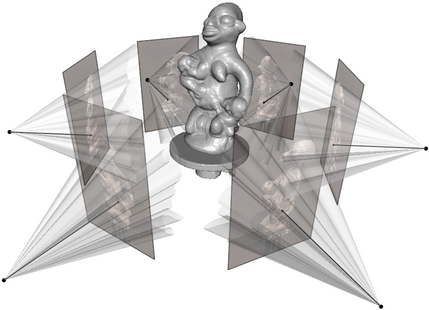
\includegraphics[height=1cm]{images/mvs.png}} &
% Texture, Specular \\
% &  \raisebox{-.5\height}{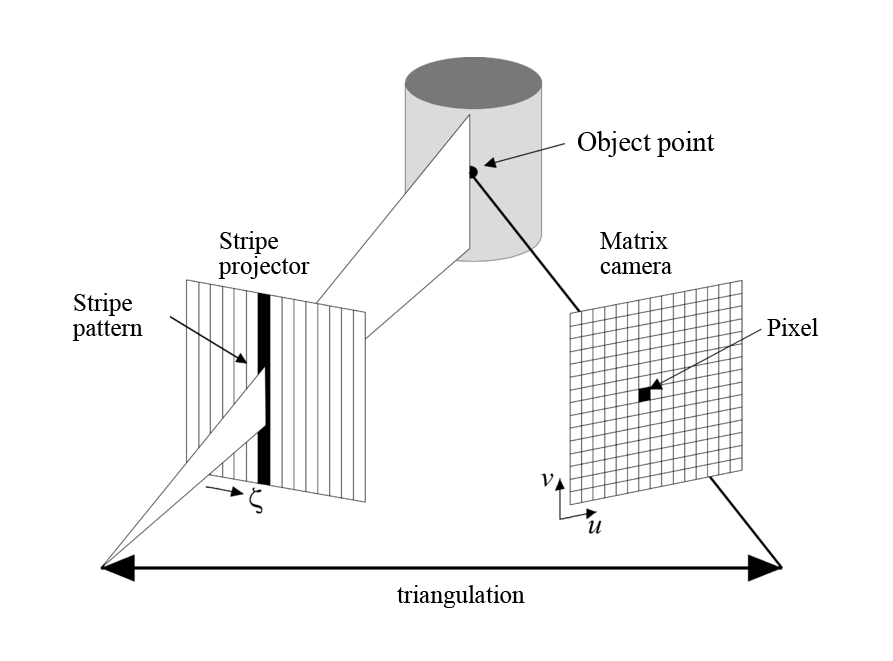
\includegraphics[height=1cm]{images/sl.jpg}} &
% Albedo, Specular \\
% \multirow{2}{*}{Shape from Intensity} & 
% \raisebox{-.5\height}{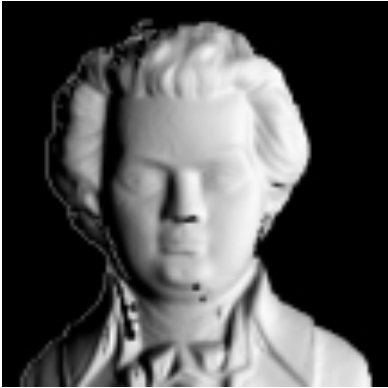
\includegraphics[height=1cm]{images/sfs.png}} &
% Albedo, Specular, Geomtry \\
% & \raisebox{-.5\height}{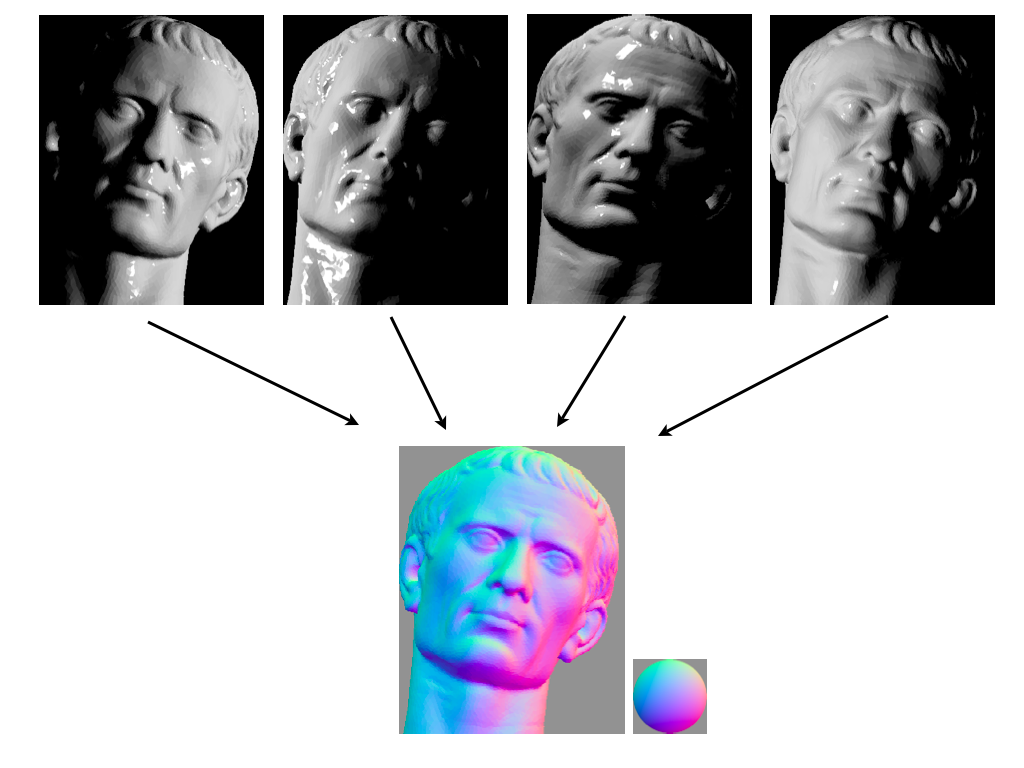
\includegraphics[height=1cm]{images/ps.png}} &
% Albedo, Geoemtry \\
% \multirow{2}{*}{Shape from Silhouette} &
% \raisebox{-.5\height}{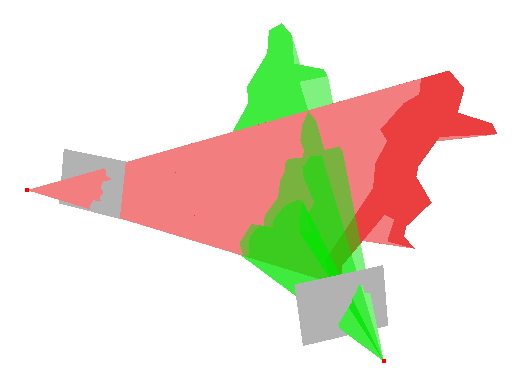
\includegraphics[height=1cm]{images/vh.jpg}} &
% Geoemtry\\
% & \raisebox{-.5\height}{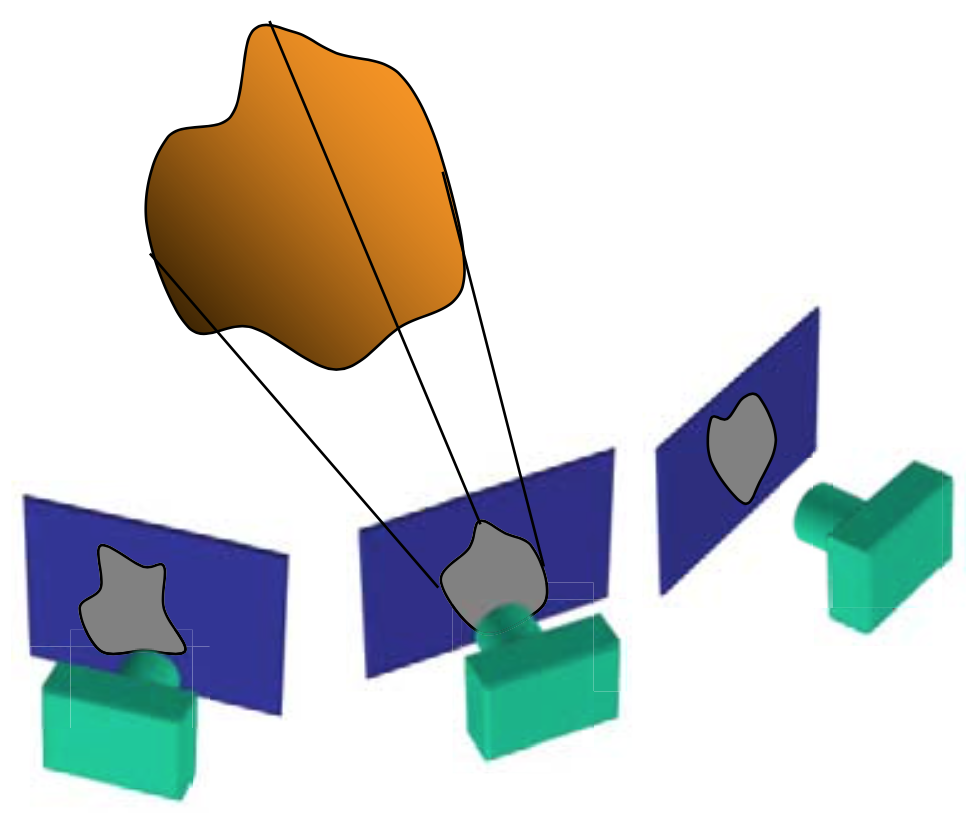
\includegraphics[height=1cm]{images/vh_1.png}} &
% Geoemtry\\
% \bottomrule
% \end{tabular}
% \end{figure}

\begin{alertblock}{Challenges}
1. Few algorithm works for objects with diverse range of properties;\\
2. The range of problem conditions under which an algorithm works is not known a priori.
\end{alertblock}

\end{frame}

%------------------------------------------------
\section{Development of Interface}
%------------------------------------------------
\begin{frame}{Overview}
\begin{figure}
\centering
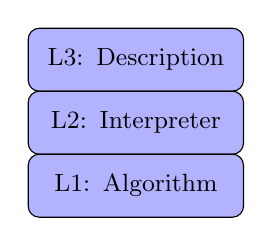
\begin{tikzpicture}[node distance=0.8cm, auto]

\node (desc) [data, font=\small] {L3: Description};
\node (interp) [data, below of=desc, font=\small] {L2: Interpreter};
\node (algo) [data, below of=interp, font=\small] {L1: Algorithm};

\end{tikzpicture}
\caption{3-layer interface to 3D reconstruction.}
\end{figure}

\begin{exampleblock}{Description}
  1. define problem space; \\
  2. describe problem condition.
\end{exampleblock}
\begin{exampleblock}{Interpreter: translate description to an appropriate algorithm.}
  Mapping: discover the relation between problem space and algorithm.
\end{exampleblock}
\begin{exampleblock}{Algorithm}
  Embed algorithms into the interface
\end{exampleblock}

\end{frame}

%------------------------------------------------
\subsection{Problem Space of 3D Reconstruction}
%------------------------------------------------
\begin{frame}{Problem space}

\begin{itemize}
\item \textit{algorithm-centered} approach categorizes algorithms based on algorithmic details, as discussed in \textbf{Related Work};
\item \textit{object-centered} taxonomy categorizes algorithms based on the problem conditions that the algorithm can reliably works under.
\end{itemize}

\begin{figure}
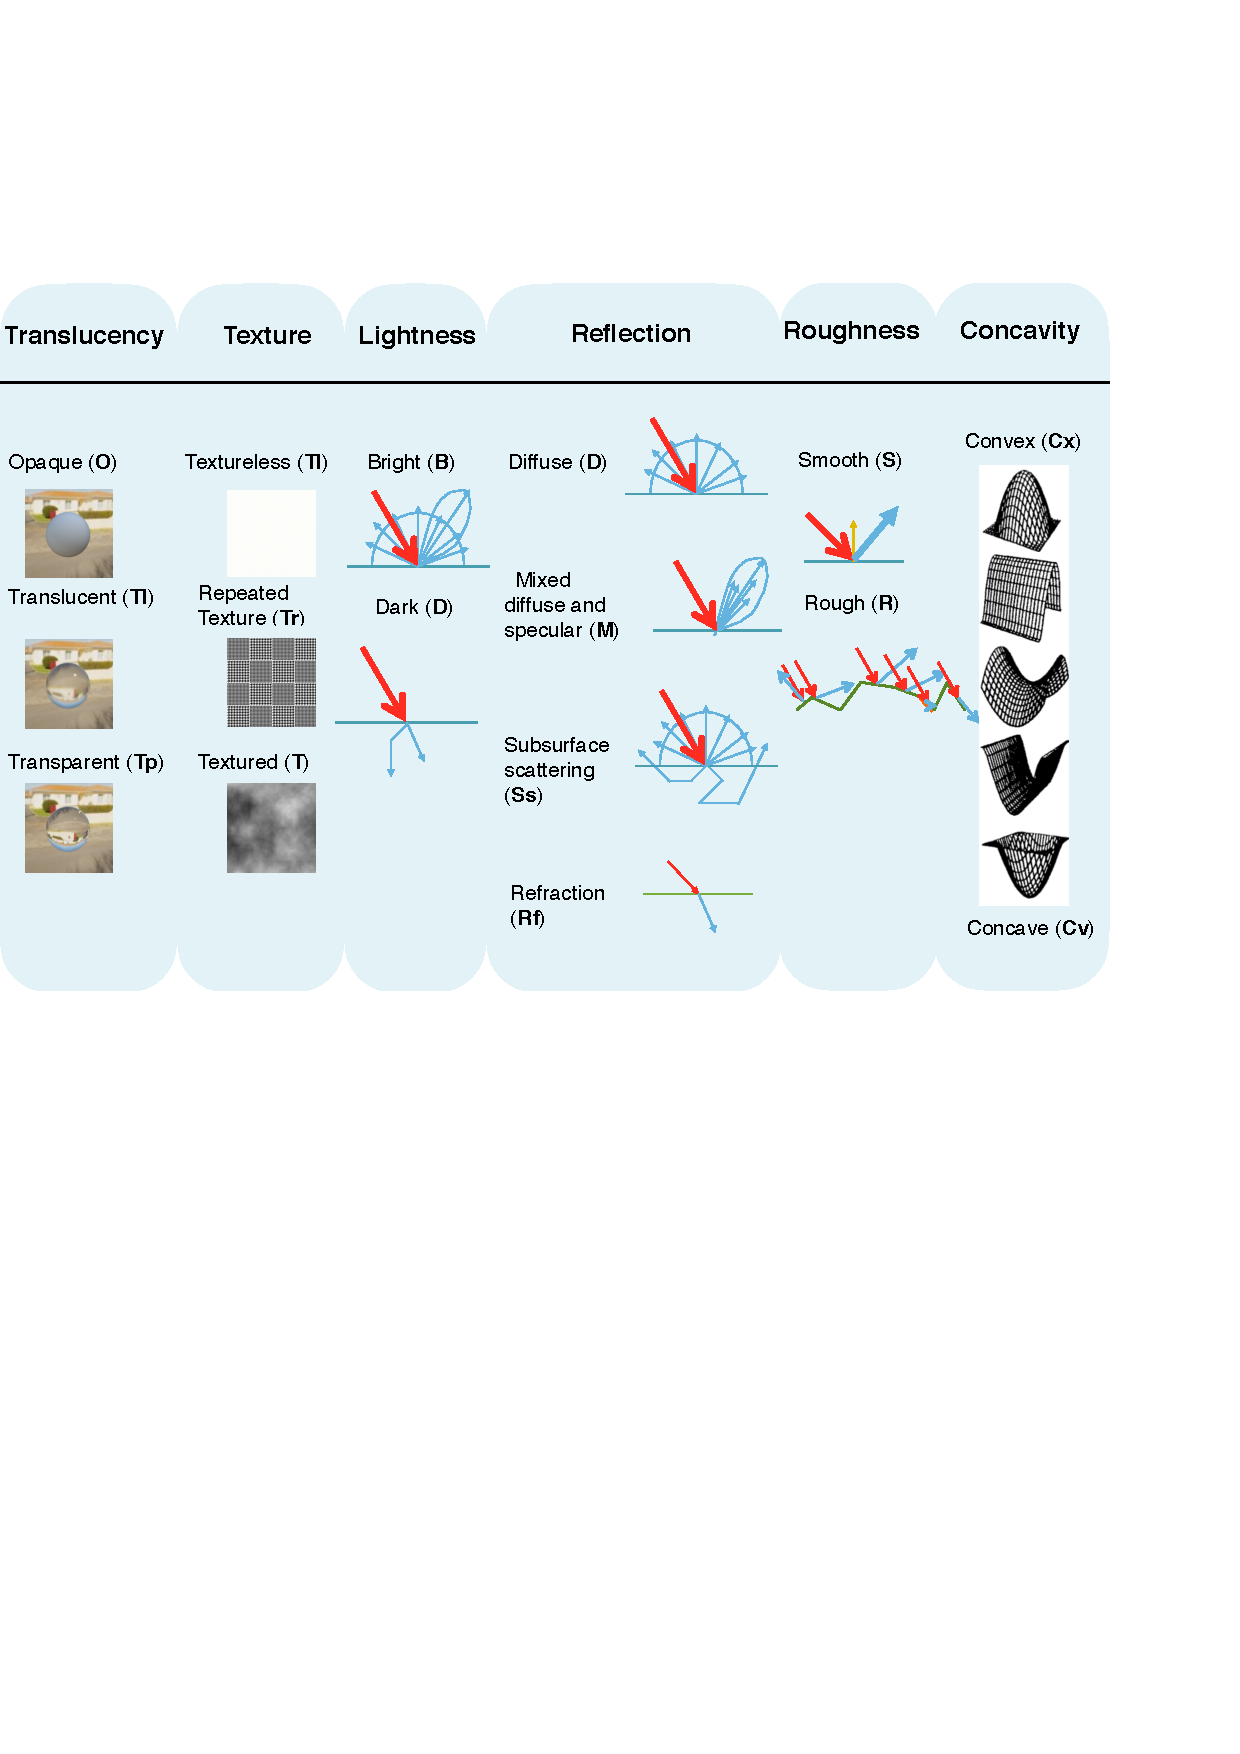
\includegraphics[width=0.7\textwidth]{prob_space/obj_class}
\end{figure}

\end{frame}

%------------------------------------------------
\begin{frame}{Problem space: four problem conditions}

Assumptions:
\begin{itemize}
\item Active methods require high surface albedo (bright), in order to demonstrate the effectiveness of these methods, we focus on bright surfaces only.
\item Diffuse is caused solely by surface roughness since sub-surface scattering is ignored.
\end{itemize}

\begin{figure}[h]
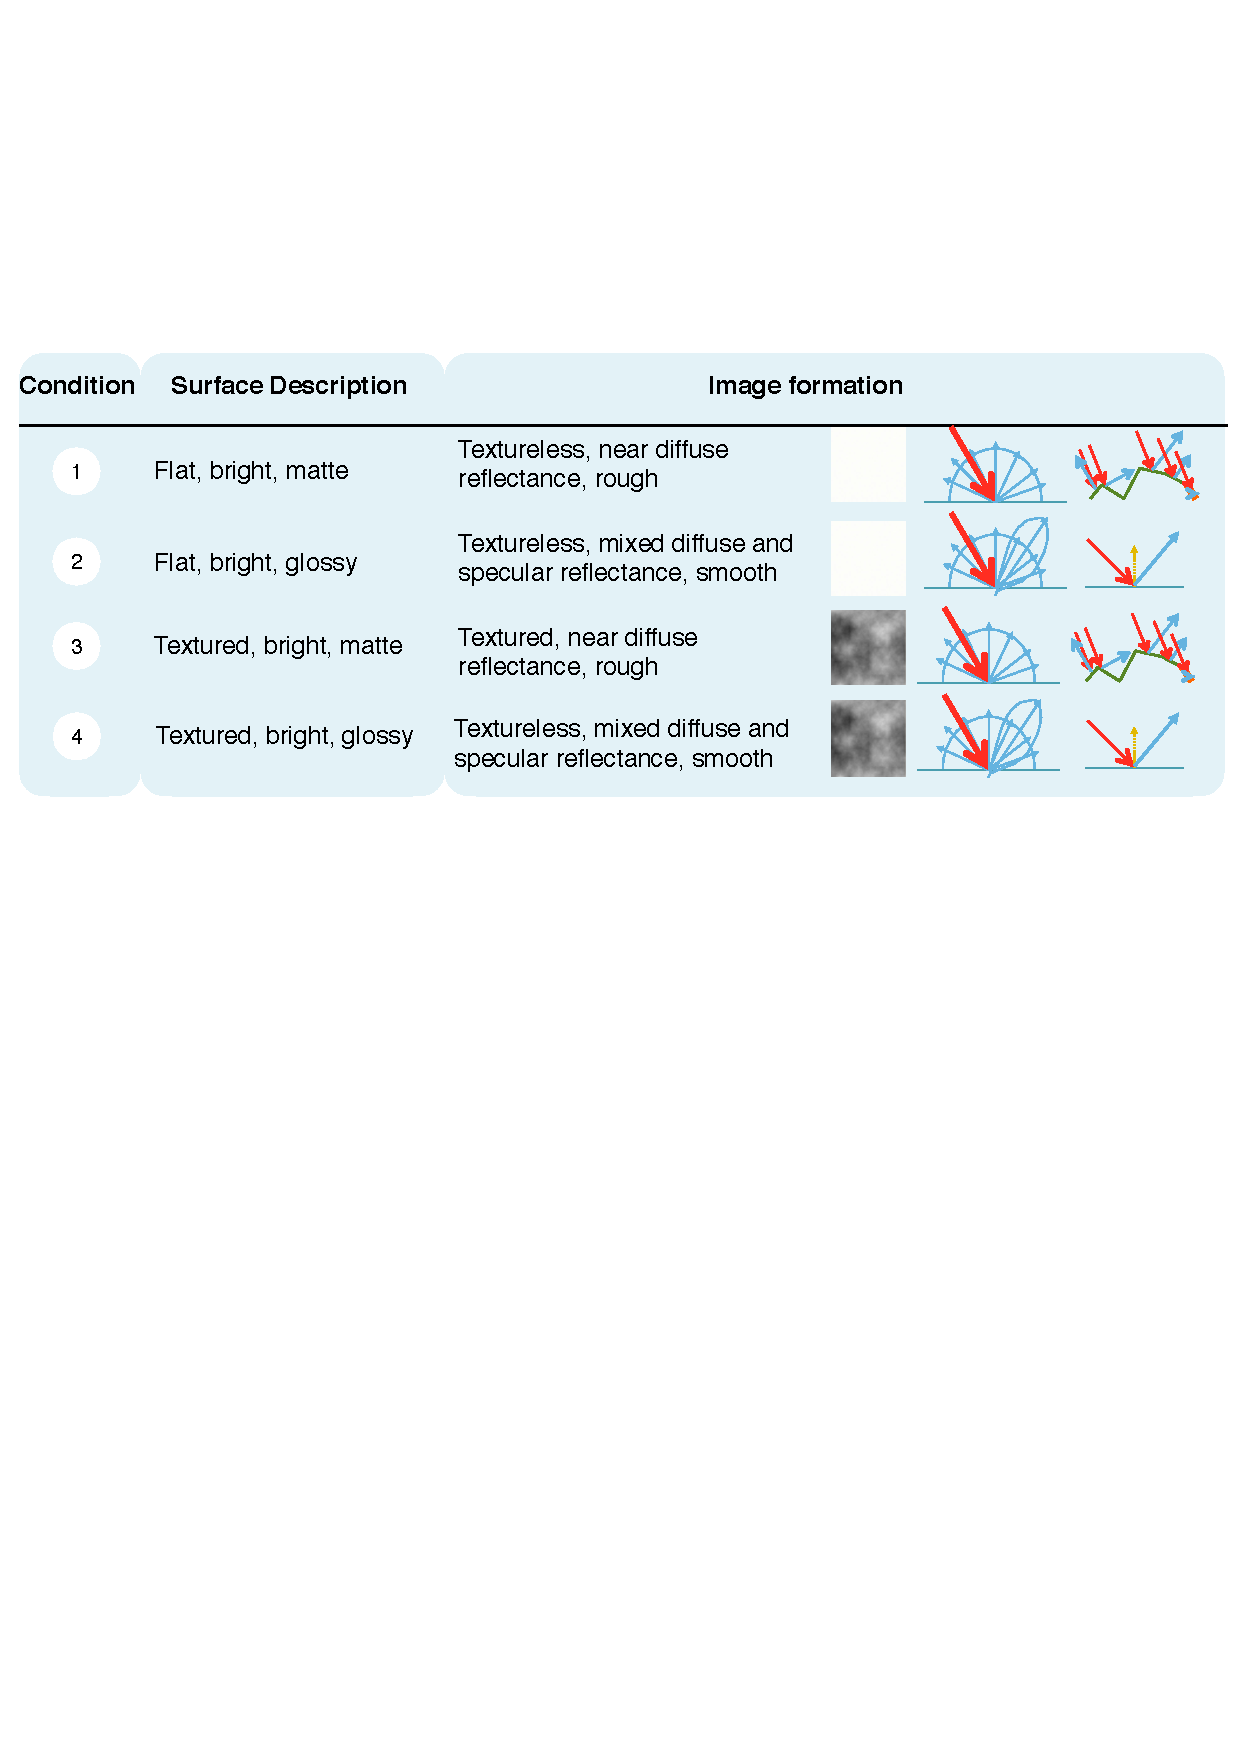
\includegraphics[width=0.7\textwidth]{prob_space/prob_cond}
\end{figure}

\end{frame}

%------------------------------------------------
\subsection{Description of 3D Reconstruction}
%------------------------------------------------
\begin{frame}{Description: model and representations}

\begin{table}[!htbp]
  \centering
  \begin{tabular}{l|ll}
  \toprule
  \textbf{Model} & \textbf{Representation}\\
  \midrule
  Texture & \textit{Texture randomness}\\
  Lightness & \textit{Diffuse albedo}\\
  Specularity & \textit{Specular reflectance}\\
  Roughness & \textit{SD of facet slopes}\\
  \bottomrule
  \end{tabular}
  \caption{Representations of the 3D reconstruction problem.}
\end{table}

\end{frame}

%------------------------------------------------
\begin{frame}{Description: expression}

We use three discrete scales to parameterize these properties: \textit{low} (0.2), \textit{medium} (0.5), and \textit{high} (0.8).
\begin{table}[!htbp]
  \centering
  \begin{tabular}{l*{4}{p{1cm}}l}
  \toprule
  \textbf{Prob cond} & Texture & Albedo & Specular & Rough & \textbf{Label}\\
  \midrule
  1 & low/med & high & low/med & high & Tl-B-D-R\\
  2 & low/med & high & high & low/med & Tl-B-M-S\\
  3 & high & high & low/med & high & T-B-D-R\\
  4 & high & high & high & low/med & T-B-M-S\\
  \bottomrule
  \end{tabular}
  \caption{Expression of the four problem conditions.}
\end{table}

\end{frame}

%------------------------------------------------
\subsection{Mapping of 3D Reconstruction}
%------------------------------------------------
\begin{frame}{Mapping}

Investigate the problem conditions under which the algorithms can reliably work.

\begin{figure}
\centering
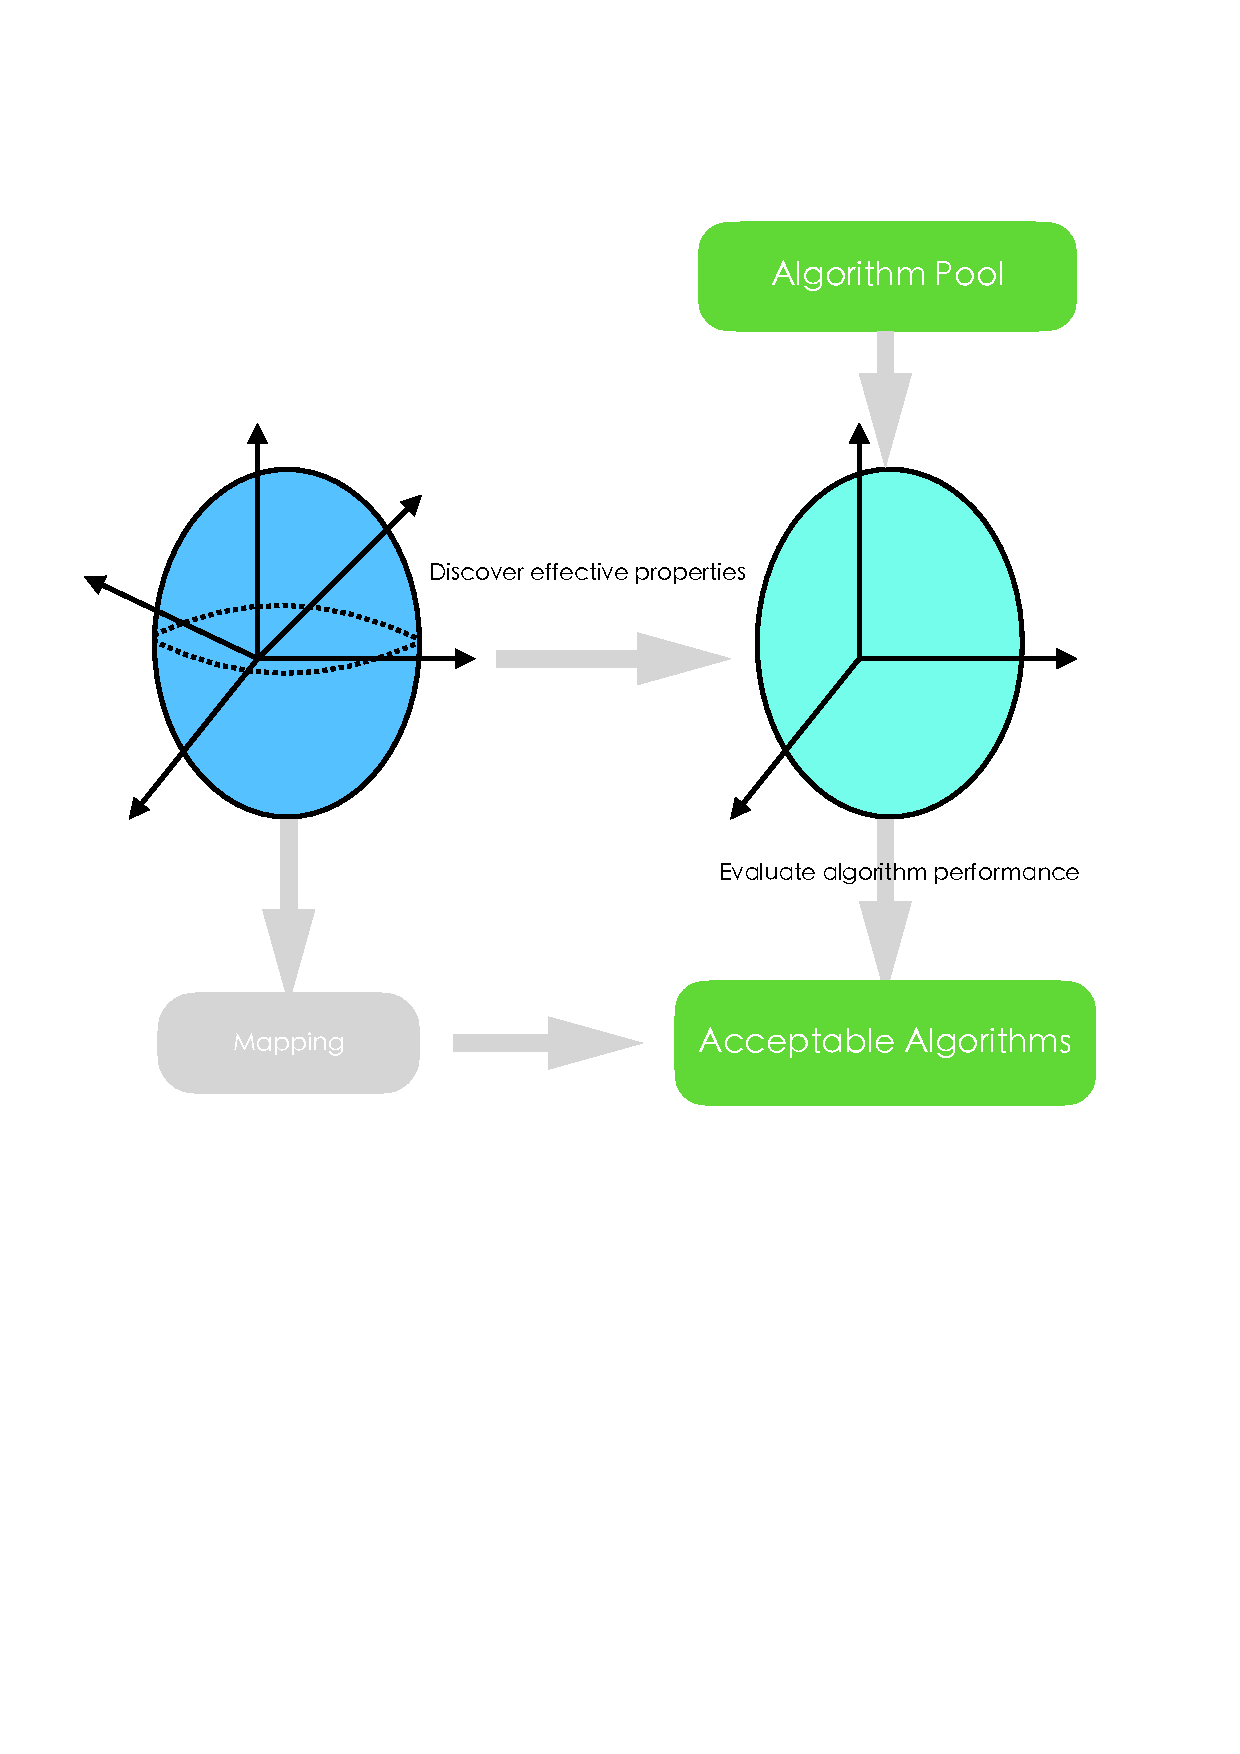
\includegraphics[width=0.6\textwidth]{images/mapping_3d_vision.pdf}
\end{figure}

% \begin{itemize}
% \item Establish the \textit{effective problem domain} (EPD): cope with large variation in material and shape.
% \item Evaluate algorithmic performance within EPD
% \item Derive mapping from problem conditions to algorithms.
% \end{itemize}

\end{frame}

%------------------------------------------------
\begin{frame}{Mapping: dataset creation}

\end{frame}

%------------------------------------------------
\begin{frame}{Mapping: notable findings 1}

\begin{figure}[!htbp]
\begin{tabular}{cc}
\includegraphics[width=0.22\textwidth]{mapping/pairwise/mvs_tex_spec}&
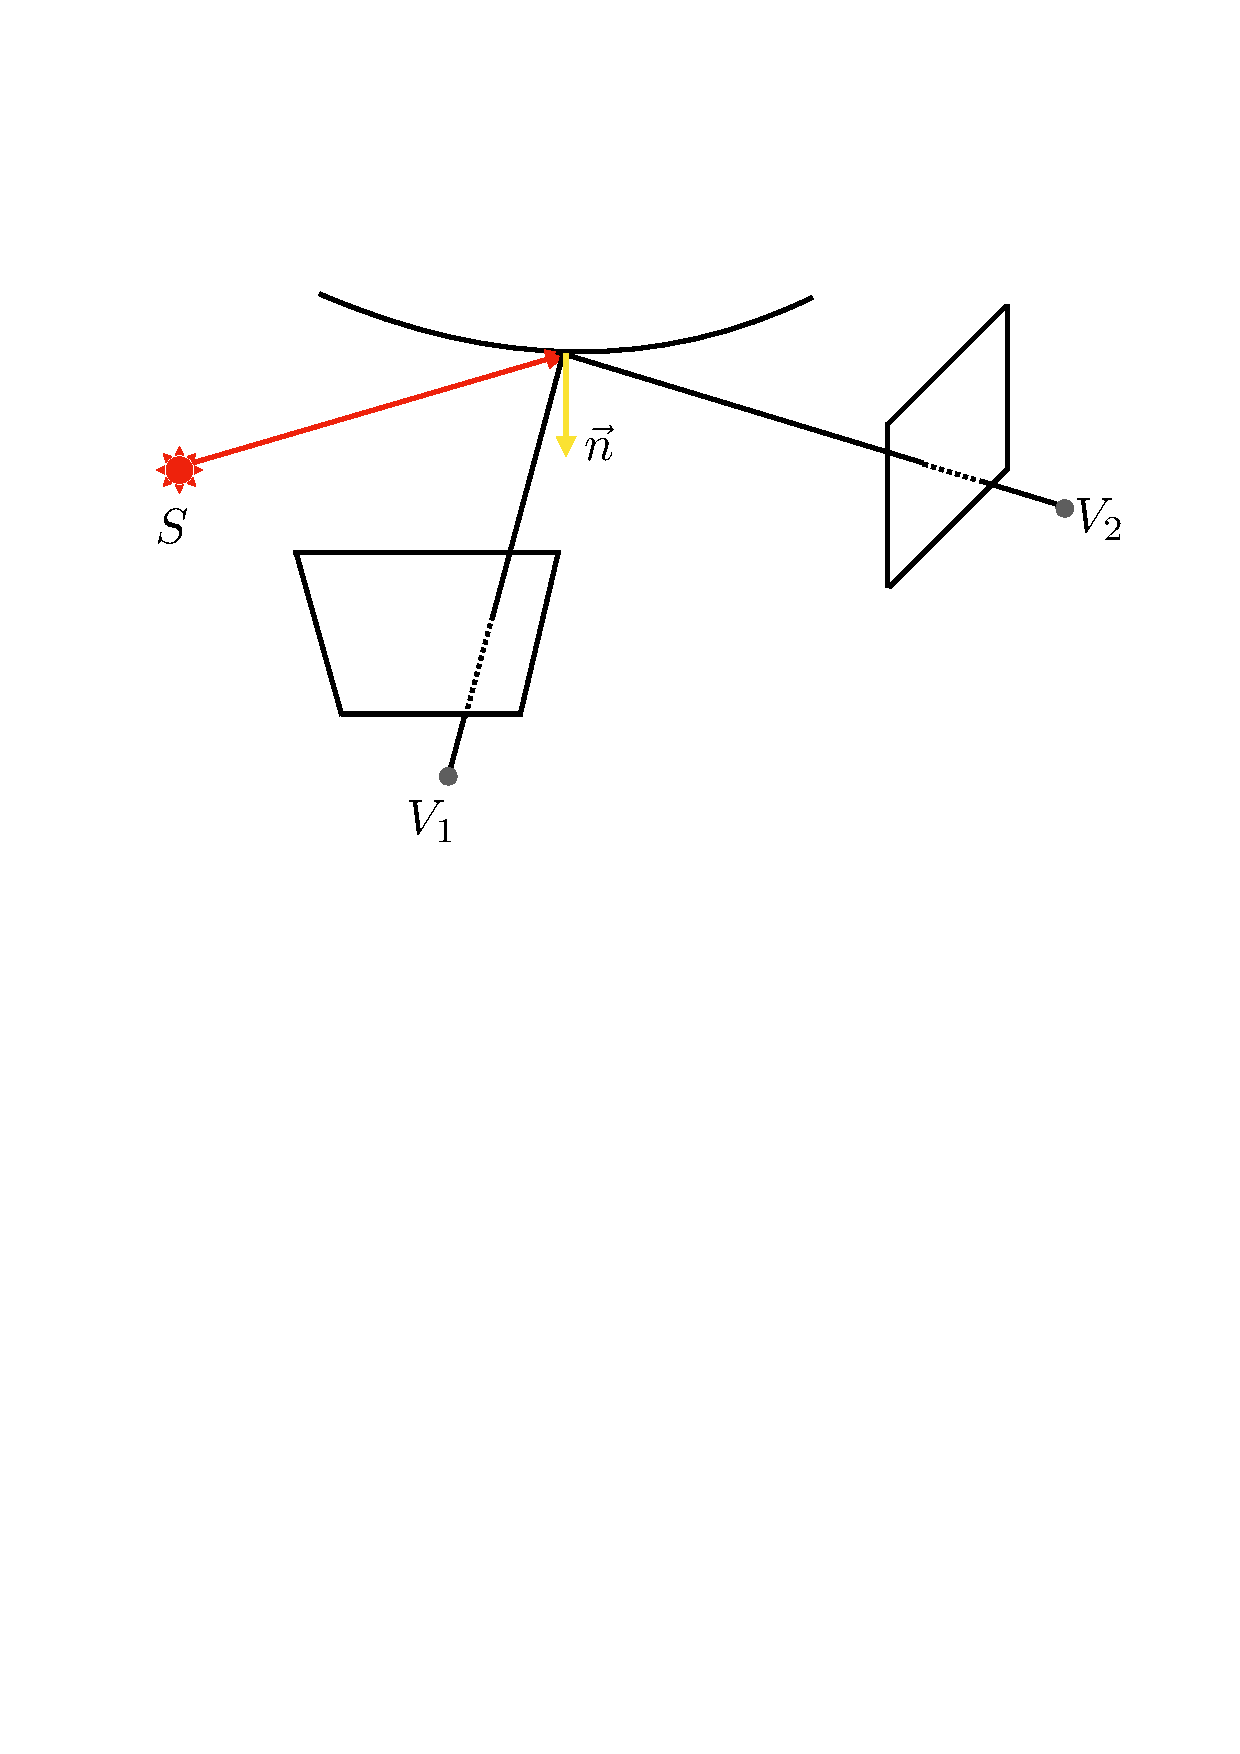
\includegraphics[width=0.22\textwidth]{mapping/mvs_spec/mvs_spec}\\
(a). Algo. performance & (b) Image formation\\
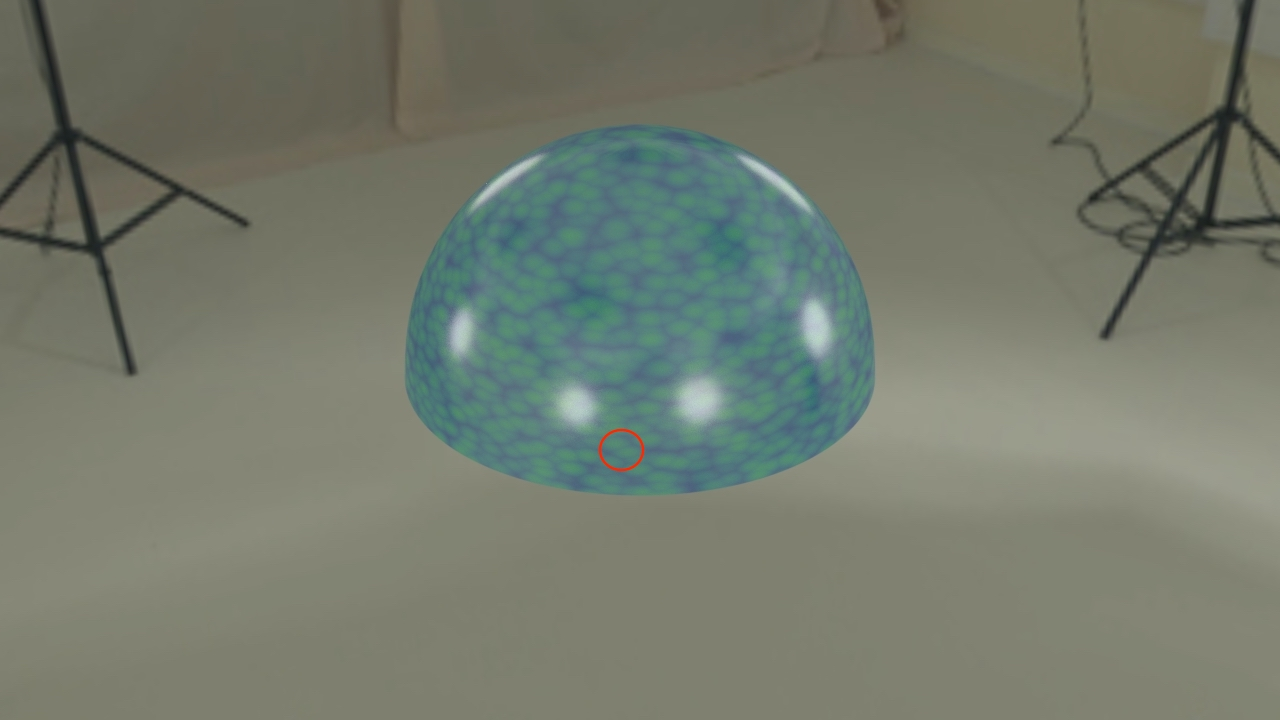
\includegraphics[width=0.22\textwidth]{mapping/mvs_spec/mvs_spec_01}&
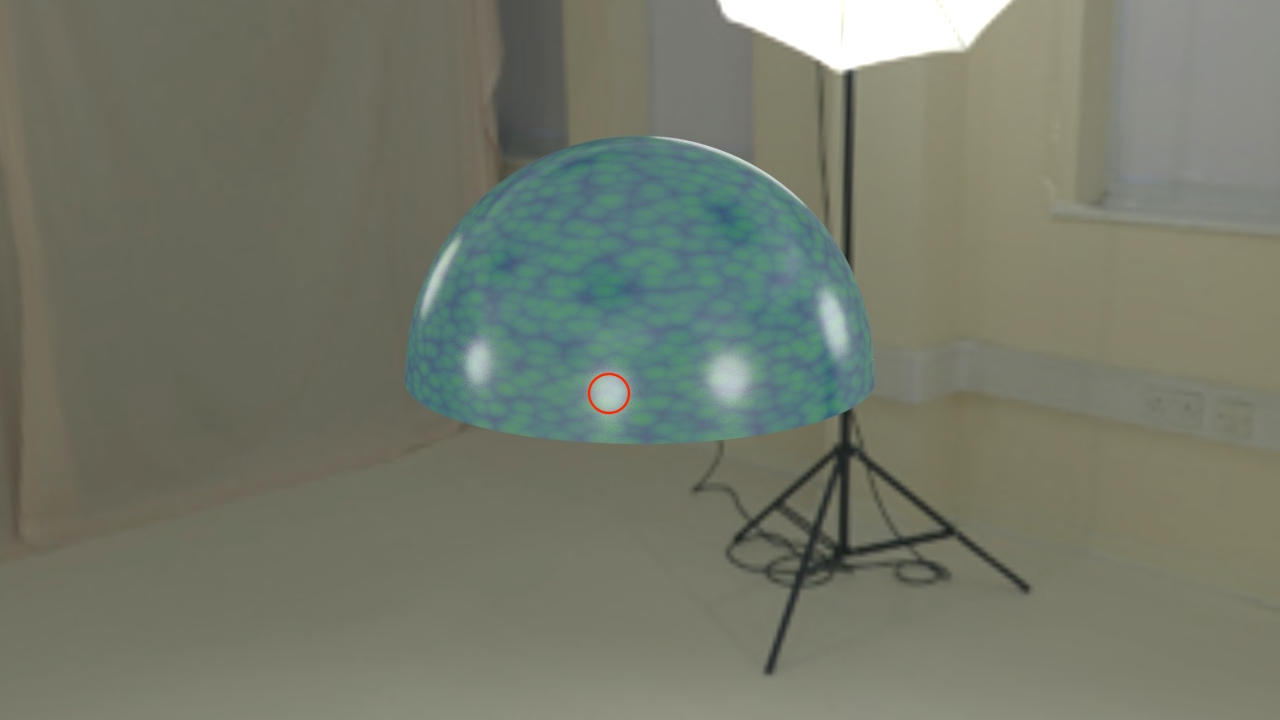
\includegraphics[width=0.22\textwidth]{mapping/mvs_spec/mvs_spec_00}\\
(c) $V_1$ & (d) $V_2$\\
\end{tabular}
\caption{(a) shows the algorithm performance w.r.t. texture and specularity. (b) shows the reflection of light off a specular surface. $V_1$ received the diffuse component while $V_2$ receives the specular component. (c), (d) shows the images observed from these two views. The specular area (red circle) observed in $V_2$ is visible in $V_1$.}
\end{figure}

\end{frame}

%------------------------------------------------
\begin{frame}{Mapping: notable findings 2}

\begin{figure}[!htbp]
\centering
\begin{tabular}{c|ccc}
  Image & Normal map & Height map & Angular error\\
  \hline\\
  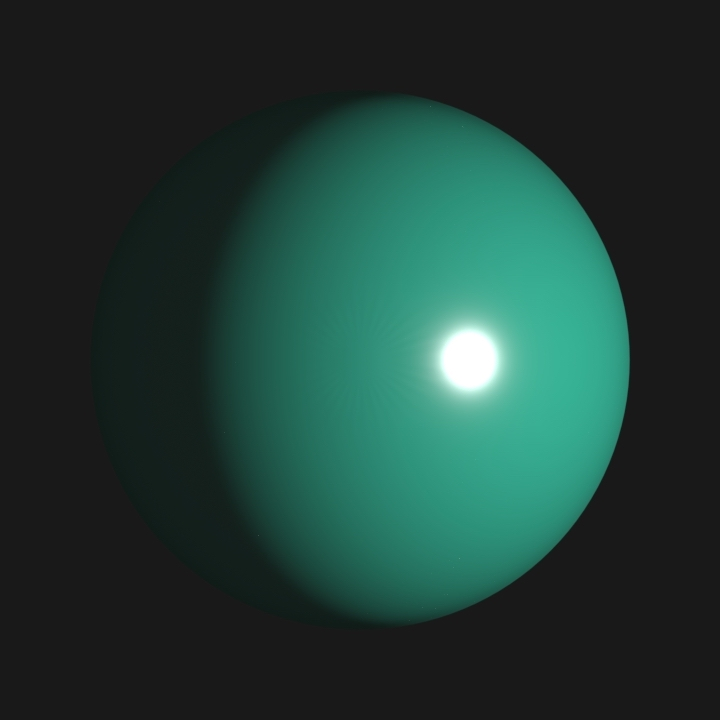
\includegraphics[width=0.12\textwidth]{mapping/ps_spec_rough/0802_0001}&
  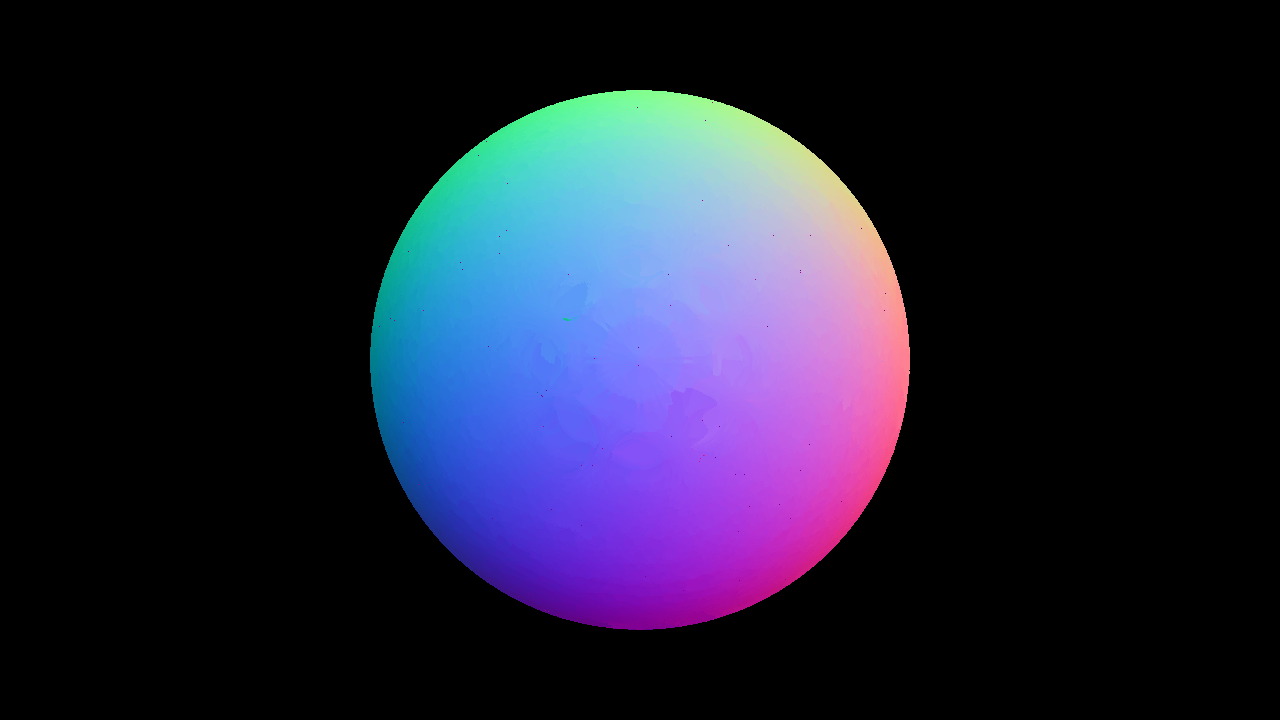
\includegraphics[width=0.12\textwidth]{mapping/ps_spec_rough/0802_normal}&
  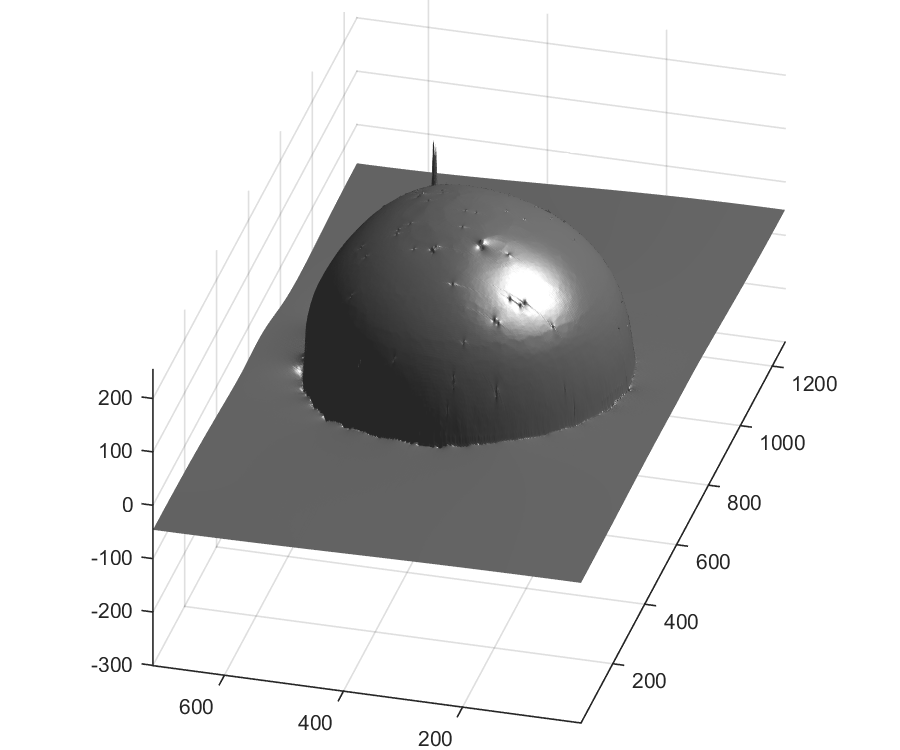
\includegraphics[width=0.15\textwidth]{images/0802_dmap}&
  \includegraphics[width=0.05\textwidth]{mapping/ps_spec_rough/0802_ang_error}\\
  & (a). rough: 0.2\\
  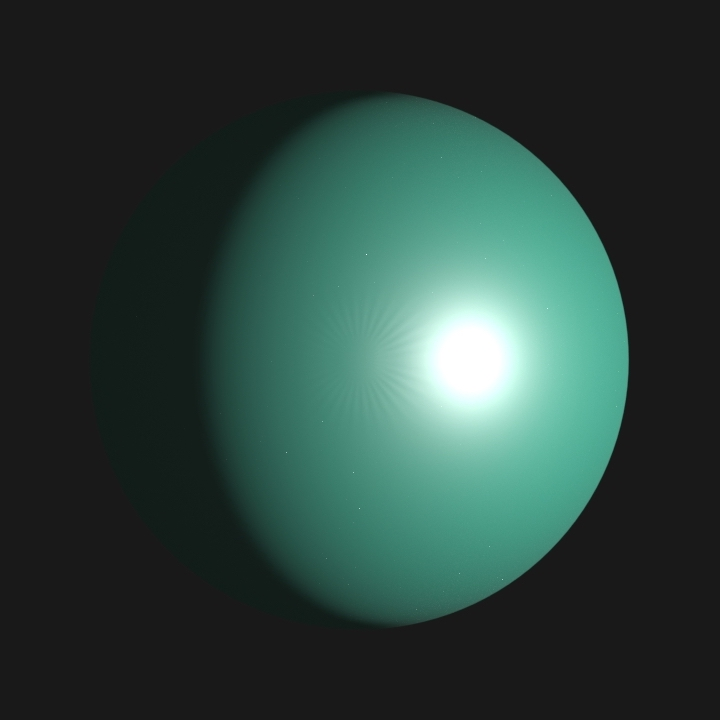
\includegraphics[width=0.12\textwidth]{mapping/ps_spec_rough/0805_0001}&
  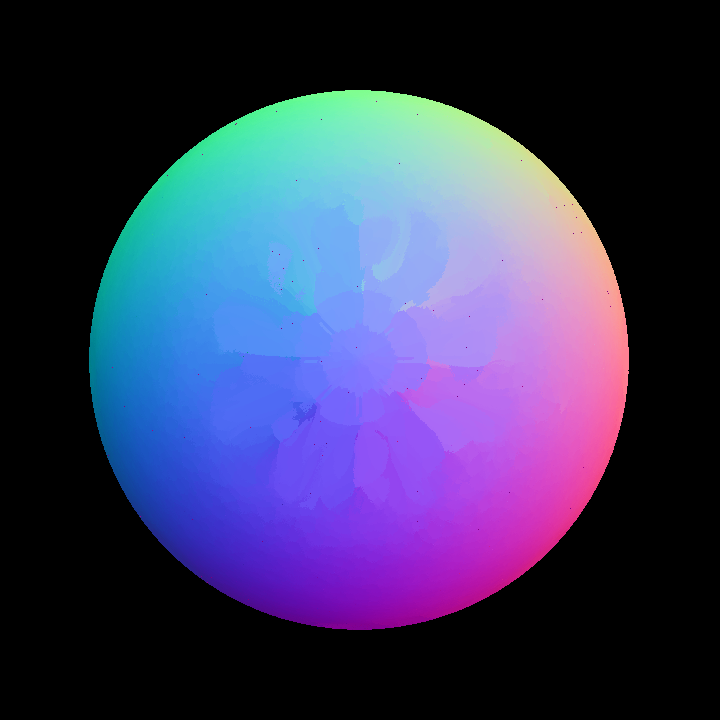
\includegraphics[width=0.12\textwidth]{mapping/ps_spec_rough/0805_normal}&
  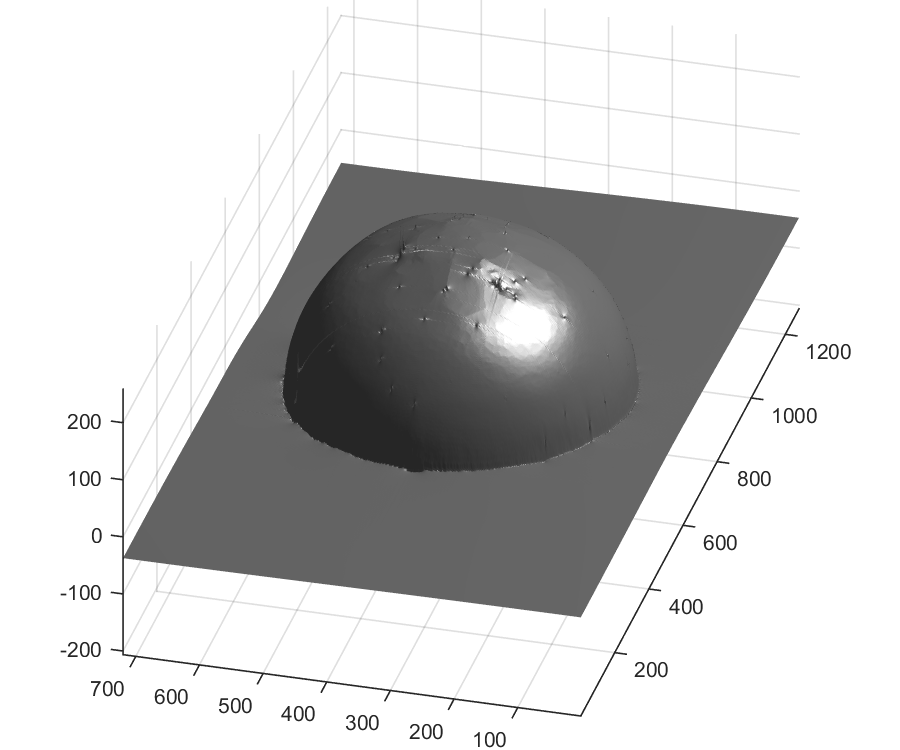
\includegraphics[width=0.15\textwidth]{images/0805_dmap}&
  \includegraphics[width=0.05\textwidth]{mapping/ps_spec_rough/0805_ang_error}\\
  & (b). rough: 0.5\\
  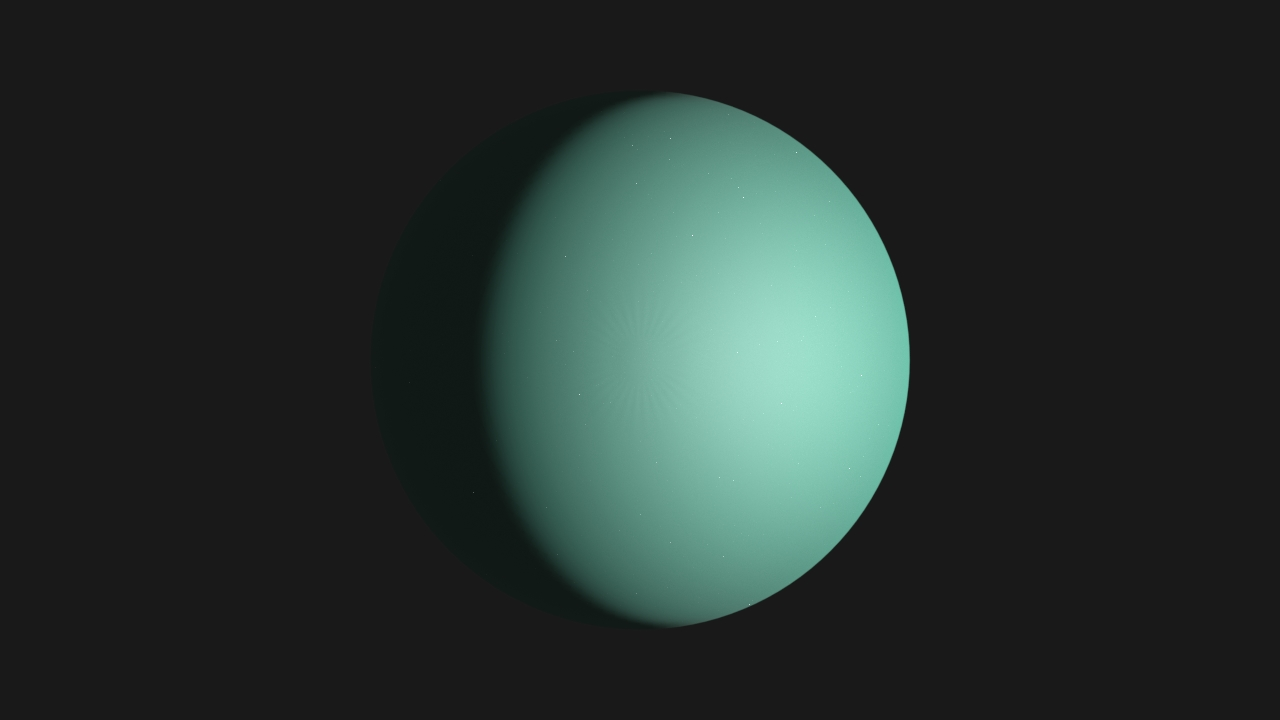
\includegraphics[width=0.12\textwidth]{mapping/ps_spec_rough/0808_0001}&
  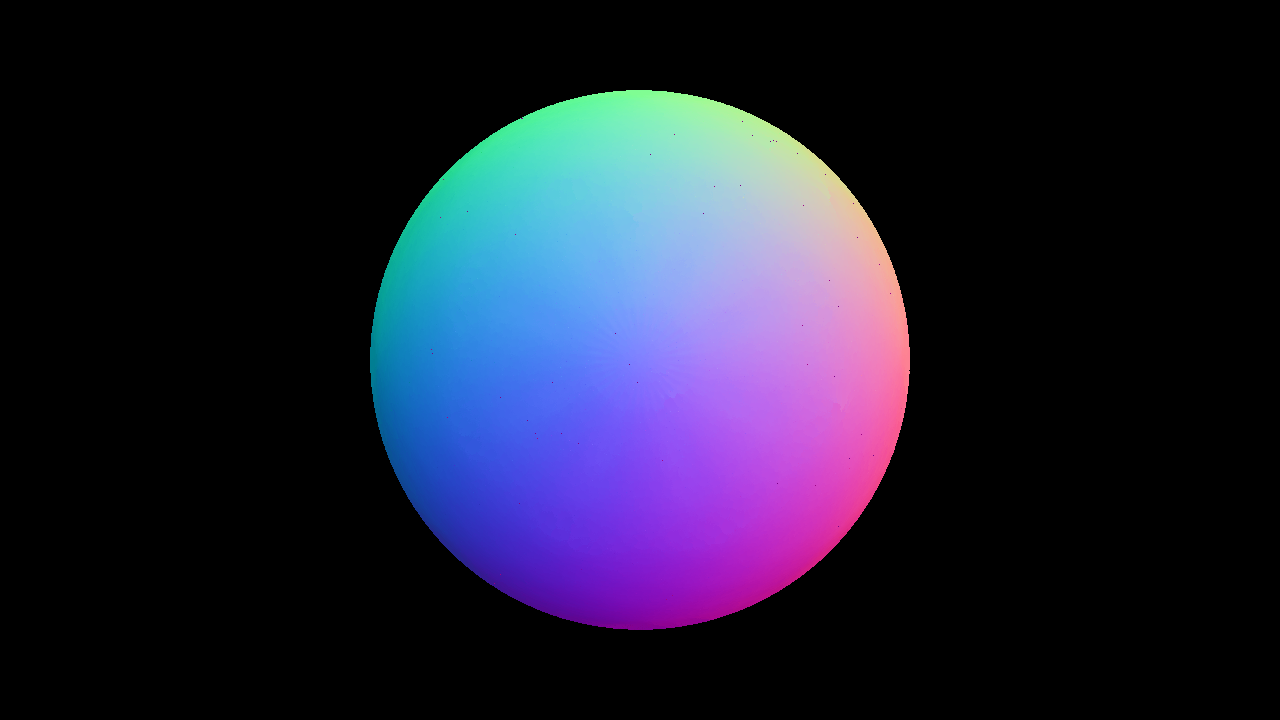
\includegraphics[width=0.12\textwidth]{mapping/ps_spec_rough/0808_normal}&
  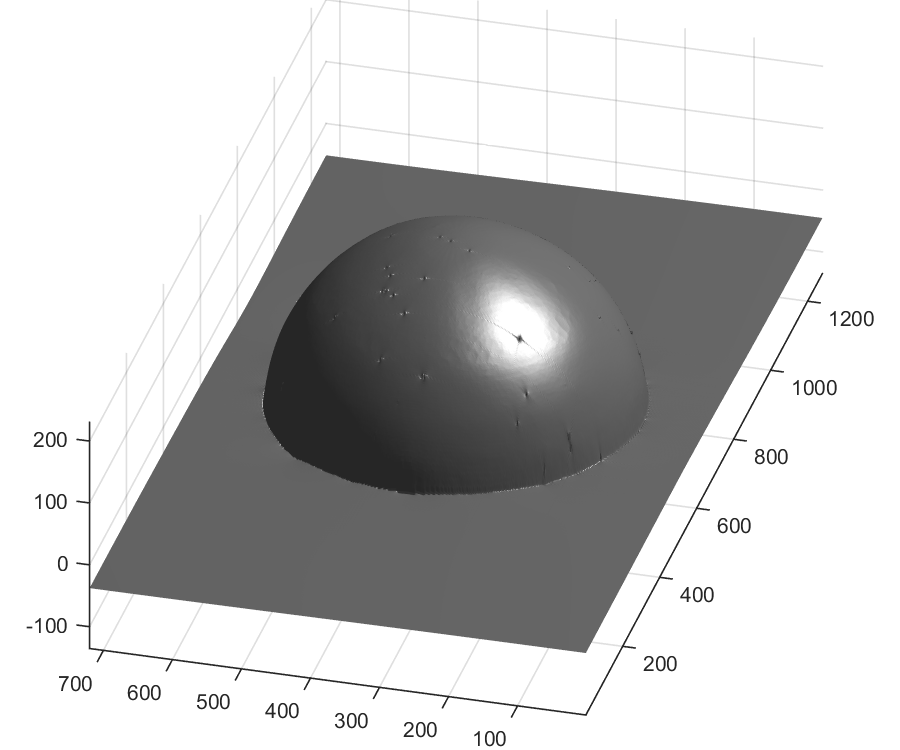
\includegraphics[width=0.15\textwidth]{images/0808_dmap}&
  \includegraphics[width=0.05\textwidth]{mapping/ps_spec_rough/0808_ang_error}\\
  & (c). rough: 0.8\\
\end{tabular}
\caption{The effect of roughness on PS. Albedo is set as 0.8, and specular is set as 0.8. (b) demonstrates that a medium level roughness would lead to worse normal estimation since it blurs the specular lobe.}
\end{figure}

\end{frame}

%------------------------------------------------
\begin{frame}{Mapping: notable findings 3}

\begin{figure}[!htbp]
\centering
\begin{tabular}{ccc}
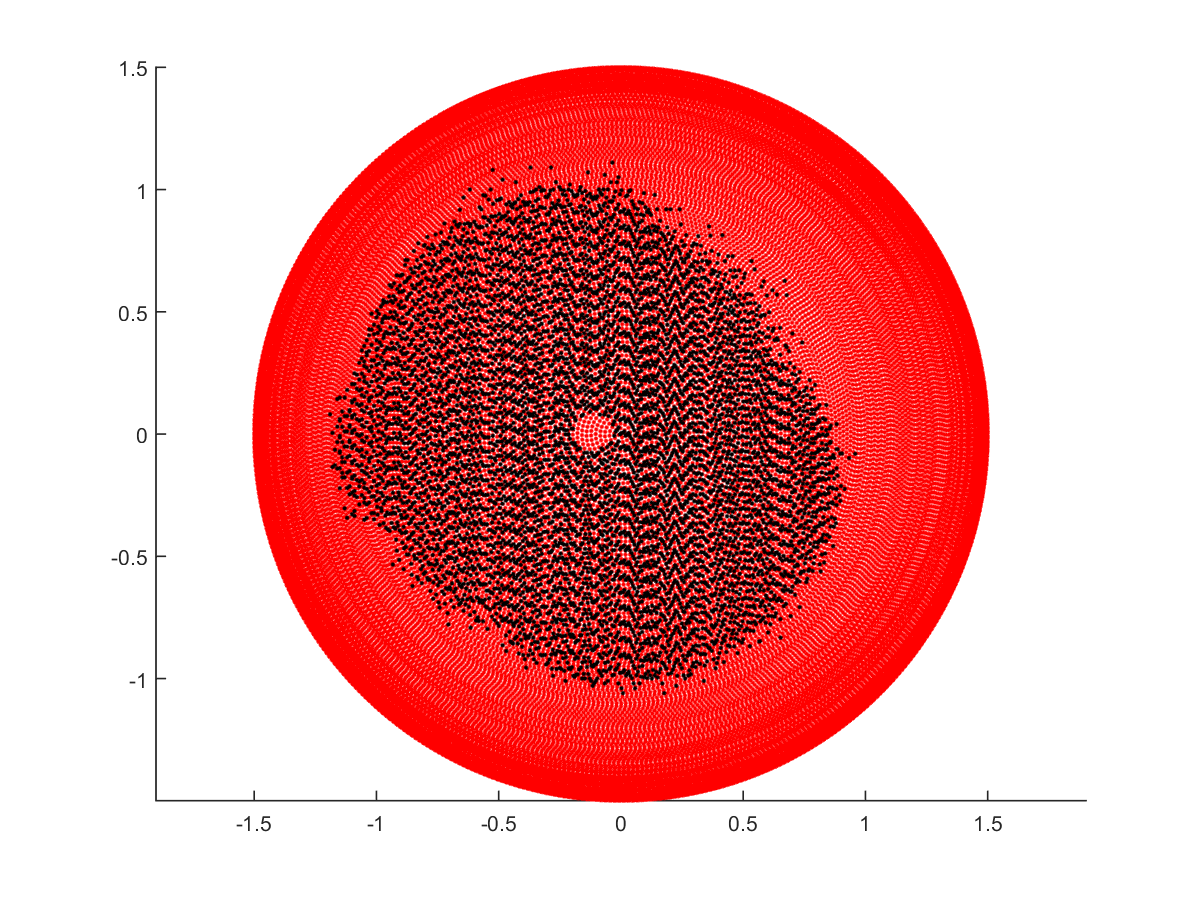
\includegraphics[width=0.25\textwidth]{trash/mapping/sl_spec_rough/sl_00050202}&
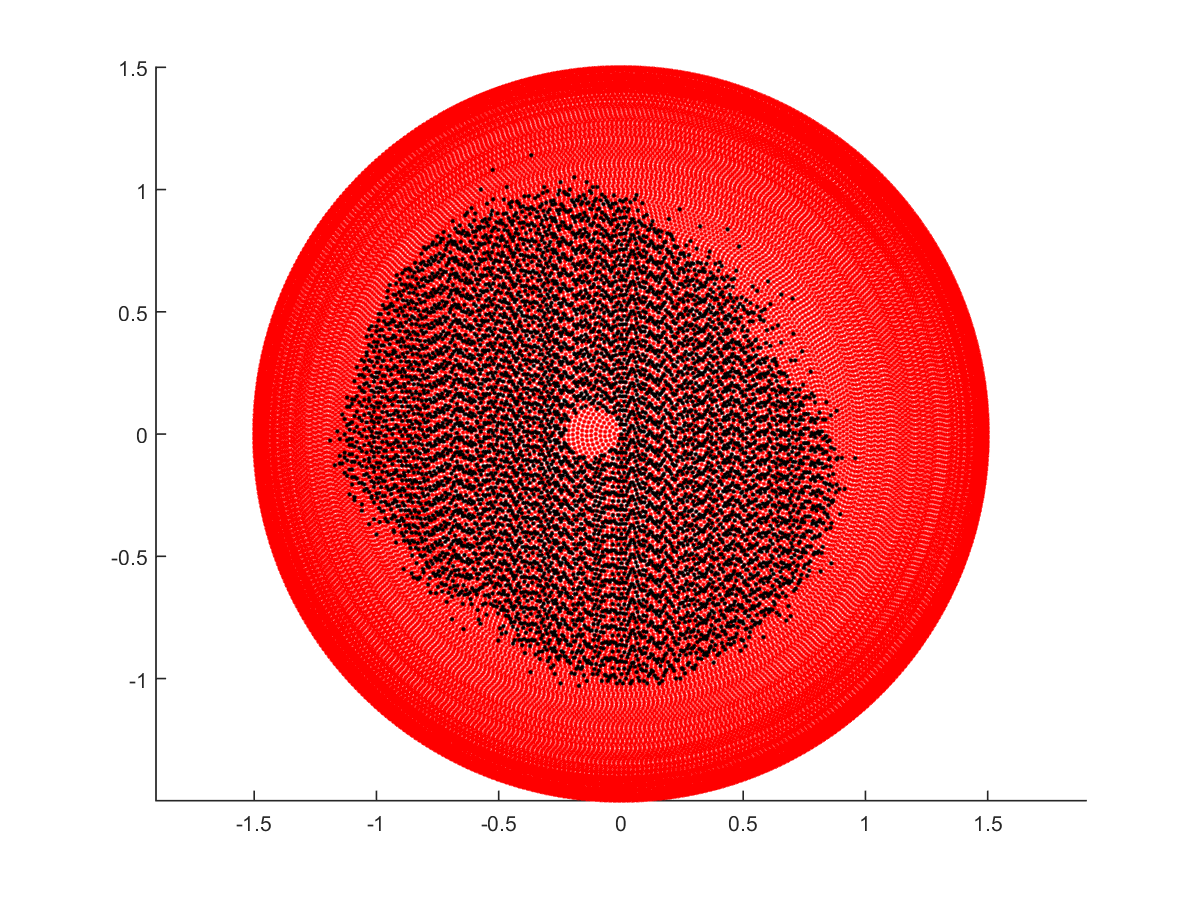
\includegraphics[width=0.25\textwidth]{trash/mapping/sl_spec_rough/sl_00050502}&
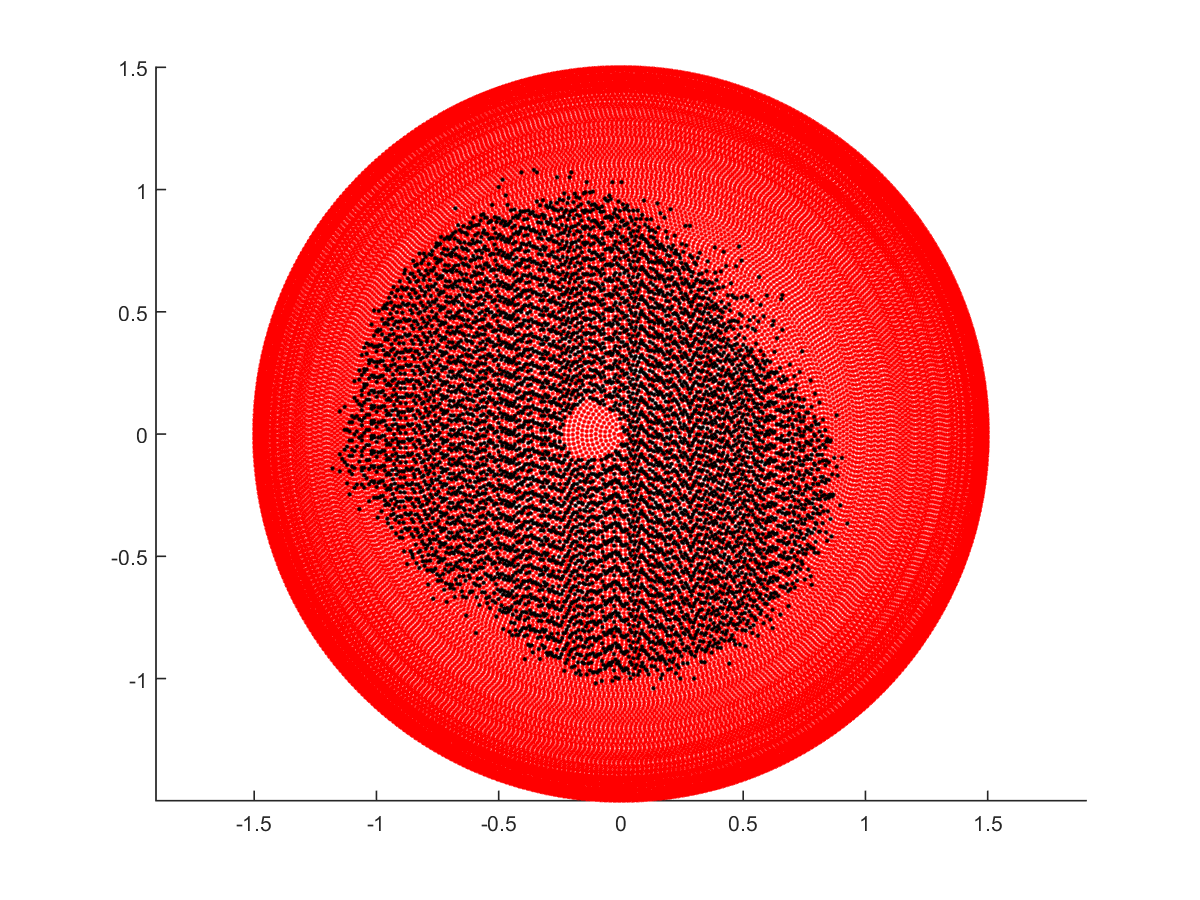
\includegraphics[width=0.25\textwidth]{trash/mapping/sl_spec_rough/sl_00050802}\\
(a) specular: 0.2 & (b) specular: 0.5 & (c) specular: 0.8\\
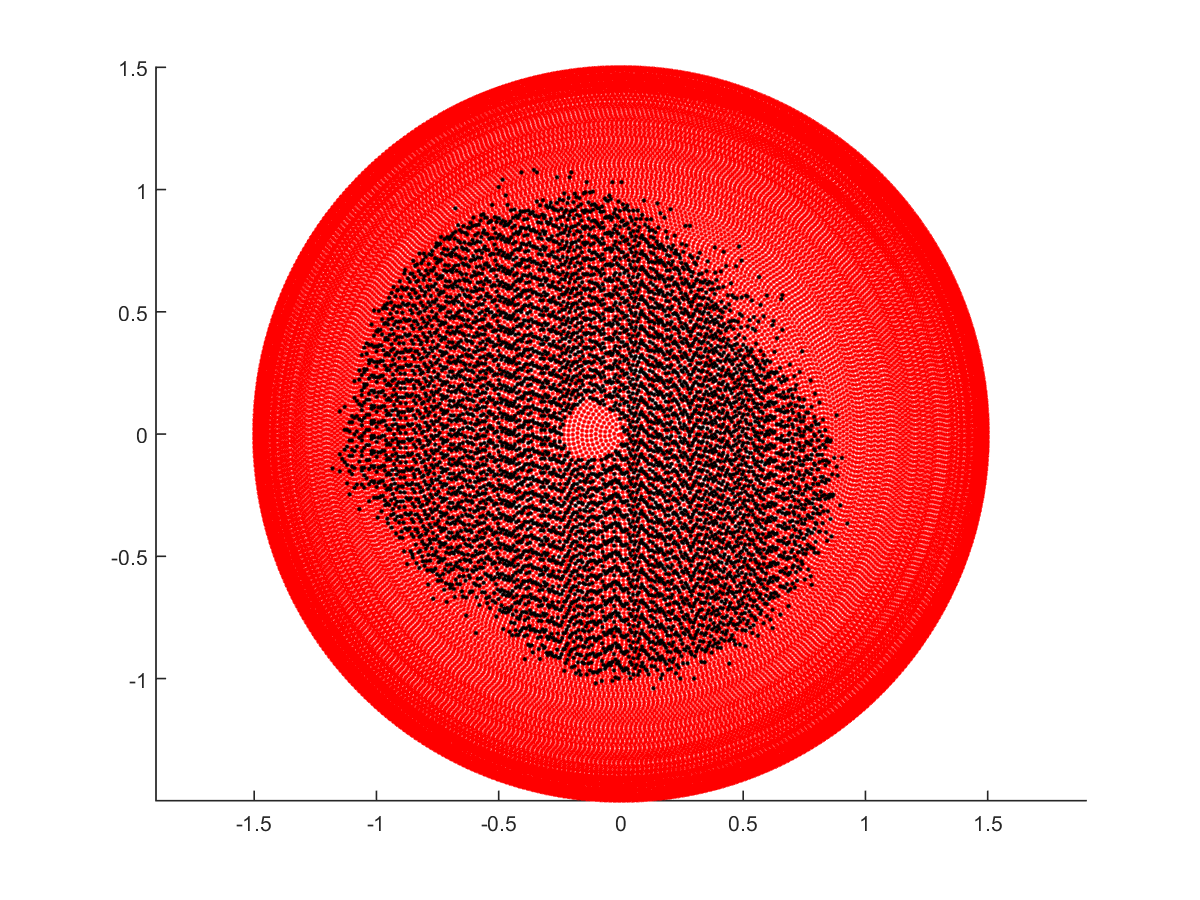
\includegraphics[width=0.25\textwidth]{trash/mapping/sl_spec_rough/sl_00050802}&
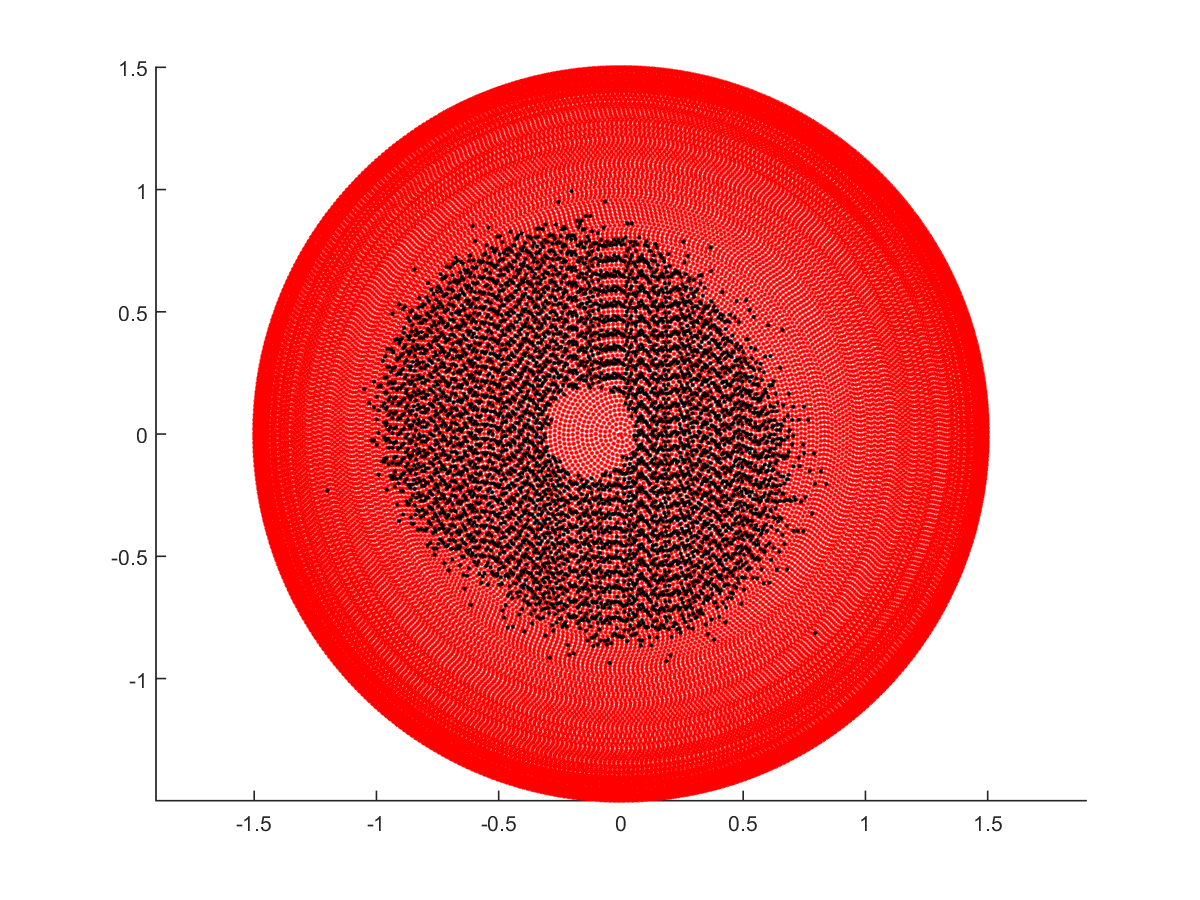
\includegraphics[width=0.25\textwidth]{trash/mapping/sl_spec_rough/sl_00050805}&
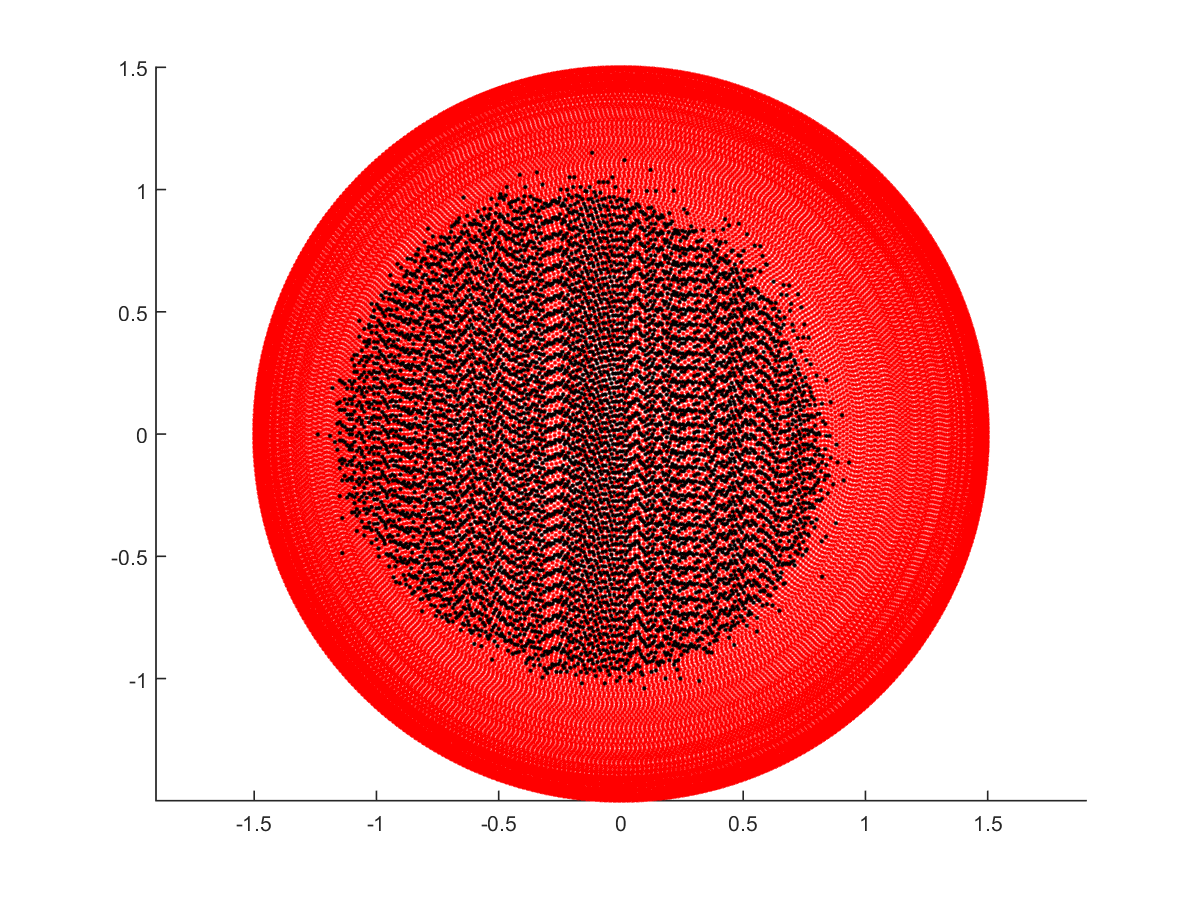
\includegraphics[width=0.25\textwidth]{trash/mapping/sl_spec_rough/sl_00050808}\\
(d) roughness: 0.2 & (e) roughness: 0.5 & (f) roughness: 0.8\\
\end{tabular}
\caption{(a)-(c): the roughness is set as 0.2, and specular has a negative effect on completeness; (d)-(e): the specular is set as 0.8, roughness has a positive effect on completeness.}
\end{figure}

\end{frame}

%------------------------------------------------
\begin{frame}{Mapping: discussion}

\begin{itemize}
\item PMVS can work on specular surfaces;
\item EPS and GSL fails on highly specular areas, and a blurred specular area causes worse results.
\end{itemize}

\end{frame}


%------------------------------------------------
\section{Evaluation of interface}
%------------------------------------------------
\begin{frame}{Interpretation: evaluation methodology}

\begin{exampleblock}{Evaluation question}
  1. Can the proof of concept interpreter return one of the best possible algorithms that achieves a successful reconstruction given the correct description? \\
  2. Can a specified description give a decent reconstruction result (baseline result)? \\
  3. Can a better description give a better reconstruction result than a worse description? \\
  4. Can a wrong description give a poor reconstruction result? \\
\end{exampleblock}

\end{frame}

%------------------------------------------------
\begin{frame}{Interpretation: evaluation methodology (cont'd)}

\begin{exampleblock}{Criteria}
  Visual comparison to results of baseline method.
\end{exampleblock}

\begin{exampleblock}{Roadmap}
  \begin{itemize}
    \item proof of concept interpreter;
    \item dataset creation;
    \item results of interpreter.
  \end{itemize}
\end{exampleblock}

\end{frame}

%------------------------------------------------
\begin{frame}{Interpretation: proof of concept interpreter}

An interpreter selects an appropriate algorithm based on description of problem condition and constraints.

\begin{figure}[!htbp]
\centering
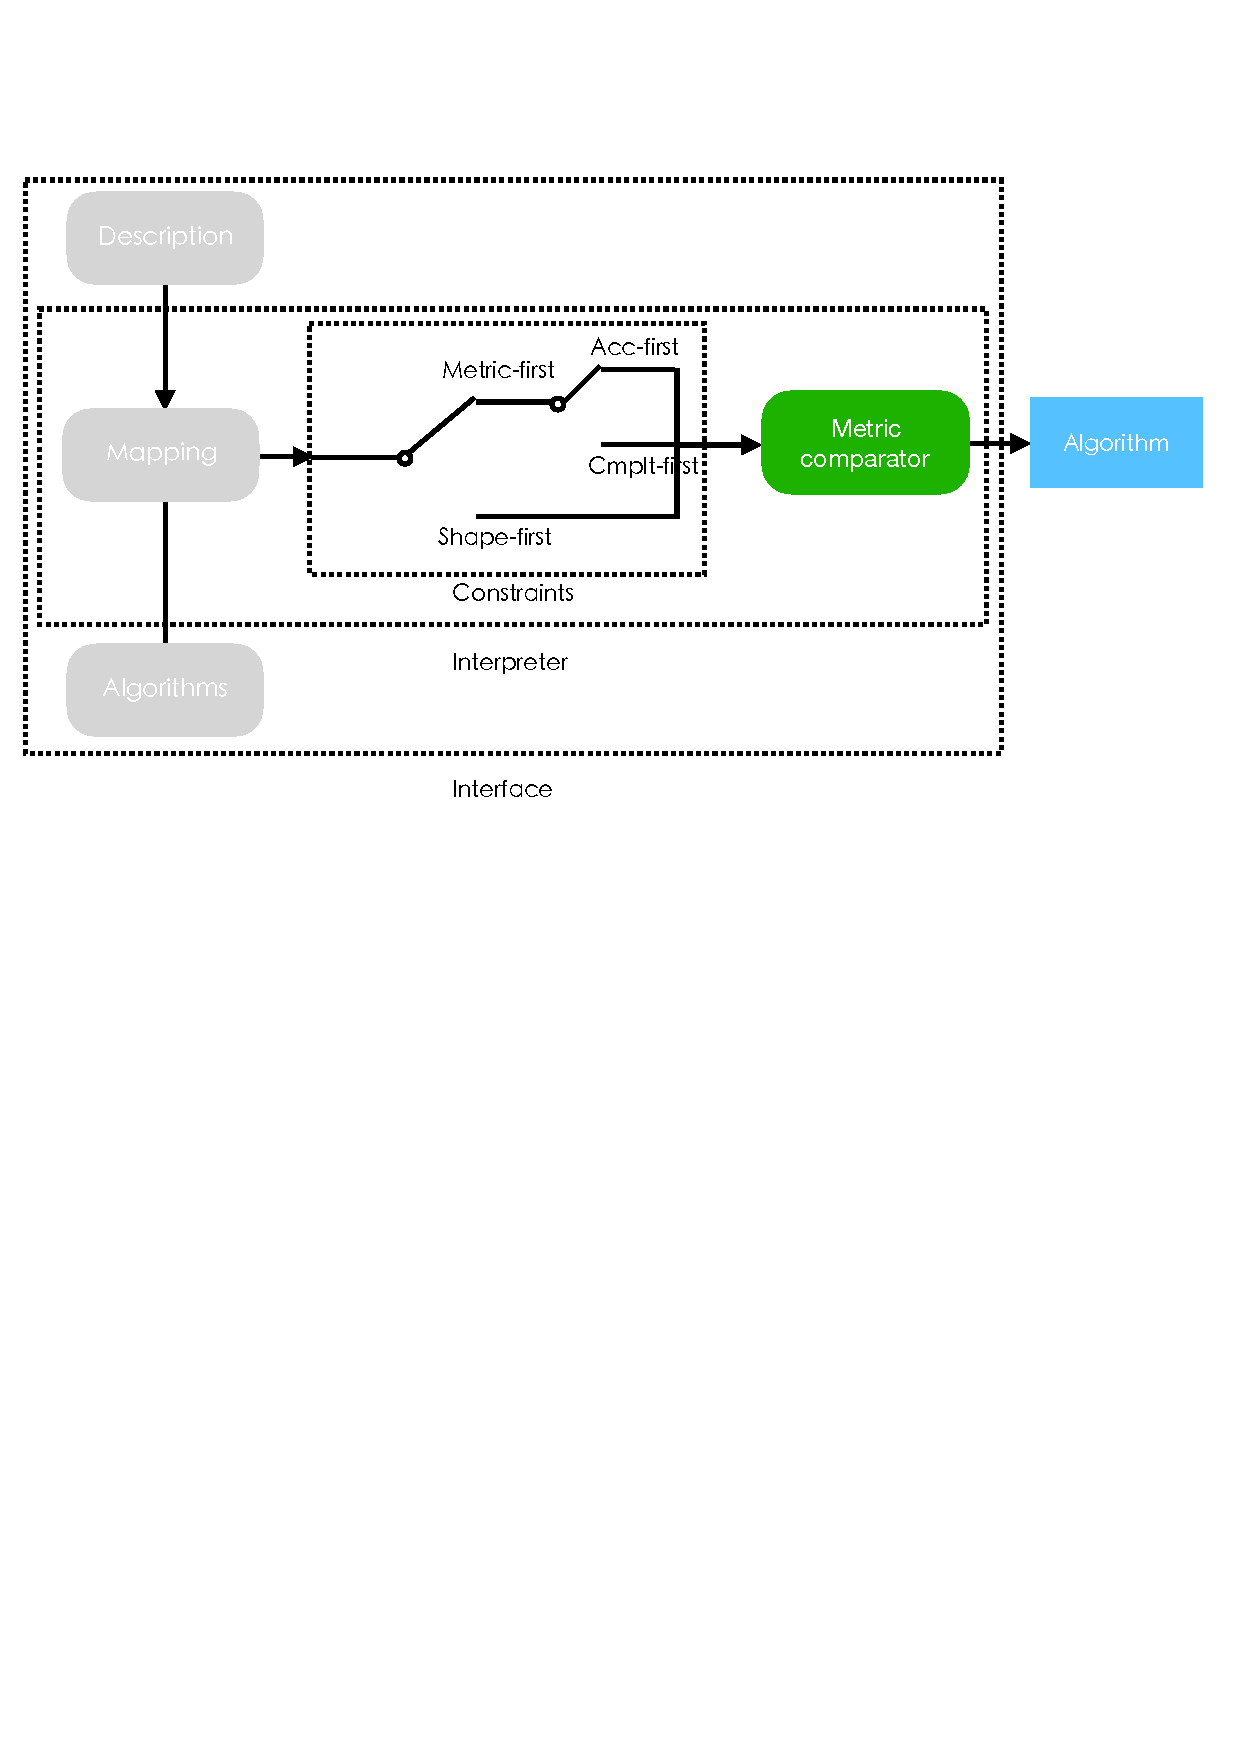
\includegraphics[width=0.8\textwidth]{interp/interpreter.pdf}
\end{figure}

\end{frame}

%------------------------------------------------
\begin{frame}{Interpretation: dataset creation}

\begin{exampleblock}{Capture}
  \begin{table}
    \begin{tabular}{l|l|l}
    method & hardware & configuration \\
    \midrule
    MVS+VH & camera & 3 heights, $30^\circ$ baseline angle \\
    PS & camera, lamp, 2 ref objs & \\
    SL & camera, projector & $10^\circ$ baseline angle\\
    \end{tabular}
  \end{table}
\end{exampleblock}

\begin{exampleblock}{Calibration}
  \begin{table}
    \begin{tabular}{l|l}
    method & calibration \\
    \midrule
    MVS+VH & focal length from EXIF, extrinsics using SfM \\
    PS & no radiometric calibration performed \\
    SL & camera-projector calibration using local homography \\
    \end{tabular}
  \end{table}
\end{exampleblock}

\end{frame}

%------------------------------------------------
\begin{frame}{Interpretation: synthetic objects}

\begin{figure}[!htbp]
\centering
\begin{tabular}{l|*{4}{p{1.5cm}}}
\toprule
prob cond\# & 1 & 2 & 3 & 4\\
\midrule
  & textureless & textureless & textured & textured\\
description & diffuse & mixed d/s & diffuse & mixed d/s\\
  & bright & bright & dark/bright & dark/bright\\
\hline
object & 
\raisebox{-.5\height}{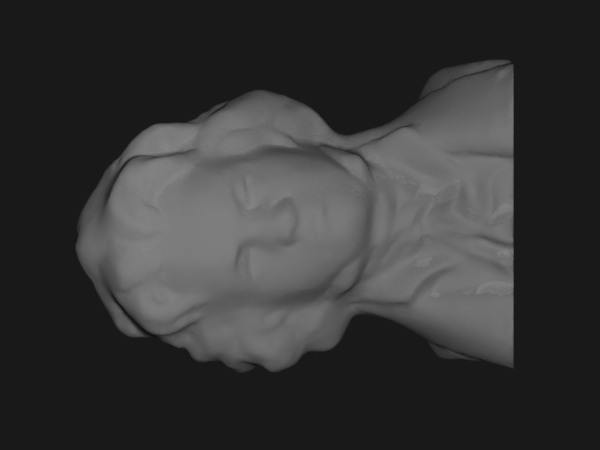
\includegraphics[width=0.15\textwidth]{interp/synth_dataset/bust}} &
\raisebox{-.5\height}{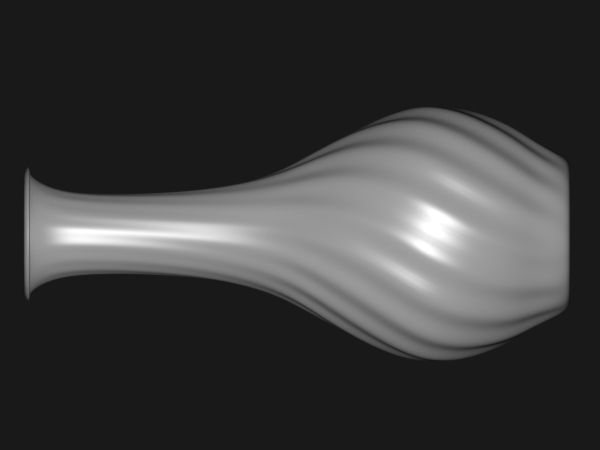
\includegraphics[width=0.15\textwidth]{interp/synth_dataset/vase0}} &
\raisebox{-.5\height}{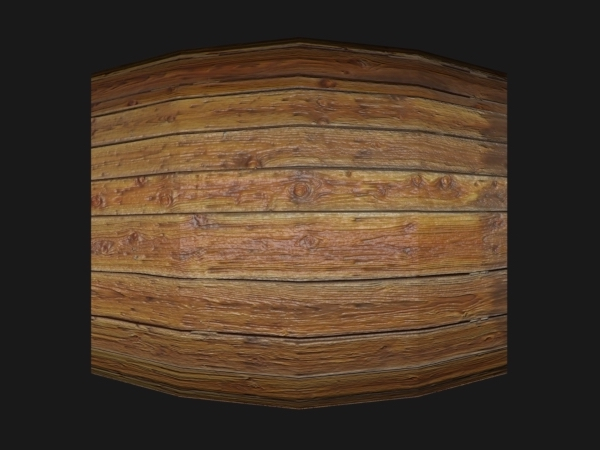
\includegraphics[width=0.15\textwidth]{interp/synth_dataset/barrel}} &
\raisebox{-.5\height}{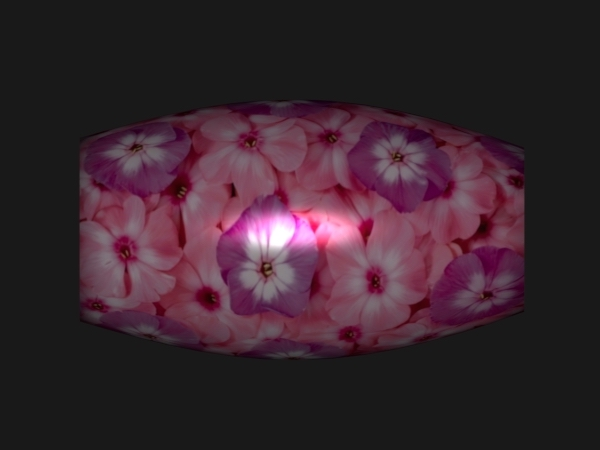
\includegraphics[width=0.15\textwidth]{interp/synth_dataset/vase1}}\\
\bottomrule
\end{tabular}
\caption{The rerepsentative synthetic objects of the four problem conditions for evaluation.}
\end{figure}

\end{frame}

%------------------------------------------------
\begin{frame}{Interpretation: evaluation of interpreter}

\begin{figure}[!htbp]
\centering
\begin{tabular}{lccccr}
\toprule
Desc \# & Bust & Vase1 & Barrel & Vase0 & Interp Algo.\\
\midrule
1 & 
\fcolorbox{green}{white}{\raisebox{-.5\height}{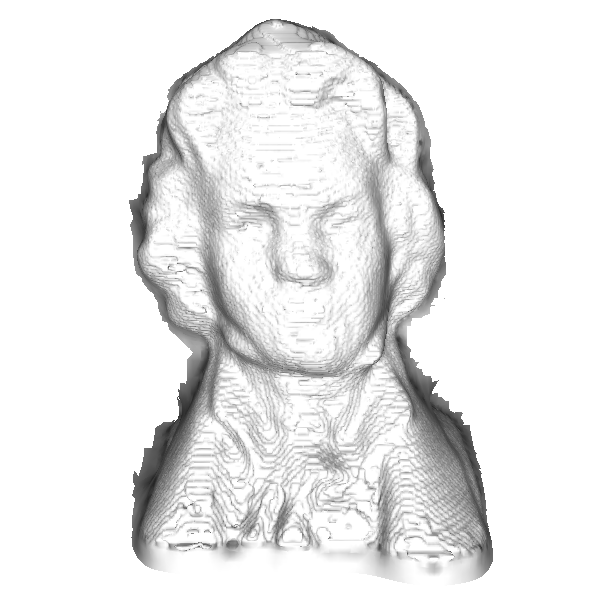
\includegraphics[width=0.1\textwidth]{interp/synth_interp/beethoven_sl}}}&
\raisebox{-.5\height}{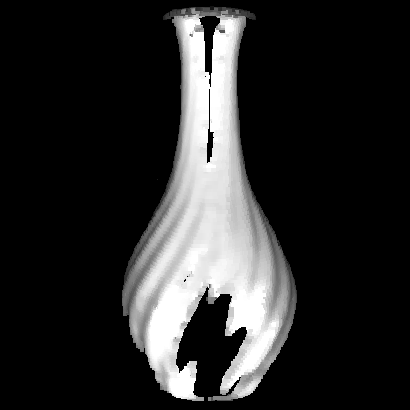
\includegraphics[width=0.1\textwidth]{interp/synth_interp/vase0_sl}}&
\raisebox{-.5\height}{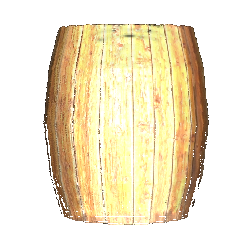
\includegraphics[width=0.1\textwidth]{interp/synth_interp/barrel_sl}}&
\raisebox{-.5\height}{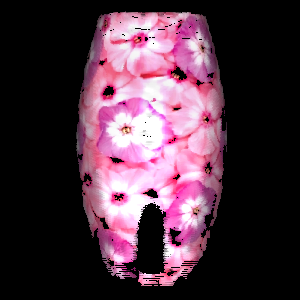
\includegraphics[width=0.1\textwidth]{interp/synth_interp/vase2_sl}}&
GSL\\
2 & 
\raisebox{-.5\height}{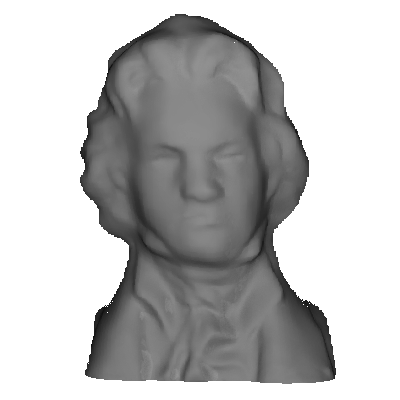
\includegraphics[width=0.1\textwidth]{interp/synth_interp/beethoven_ps}}&
\fcolorbox{green}{white}{\raisebox{-.5\height}{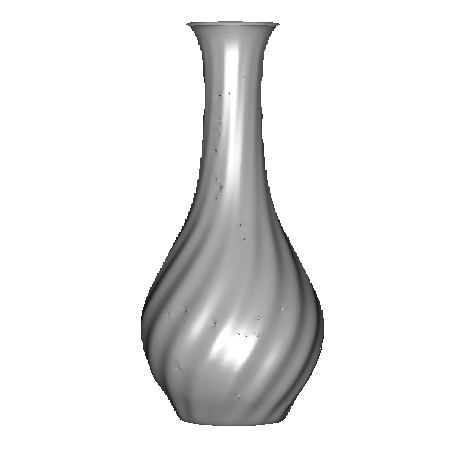
\includegraphics[width=0.1\textwidth]{interp/synth_interp/vase0_ps}}}&
\raisebox{-.5\height}{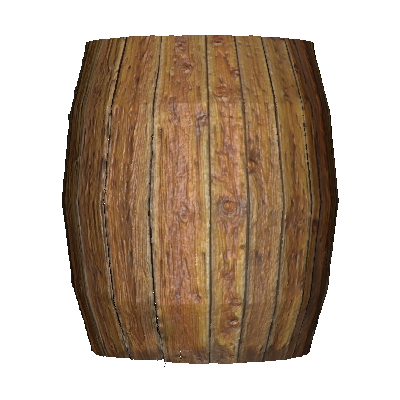
\includegraphics[width=0.1\textwidth]{interp/synth_interp/barrel_ps}}&
\raisebox{-.5\height}{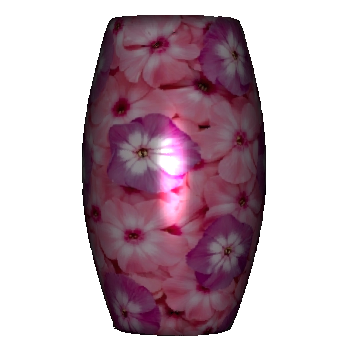
\includegraphics[width=0.1\textwidth]{interp/synth_interp/vase2_ps}}&
EPS\\
3 & 
\raisebox{-.5\height}{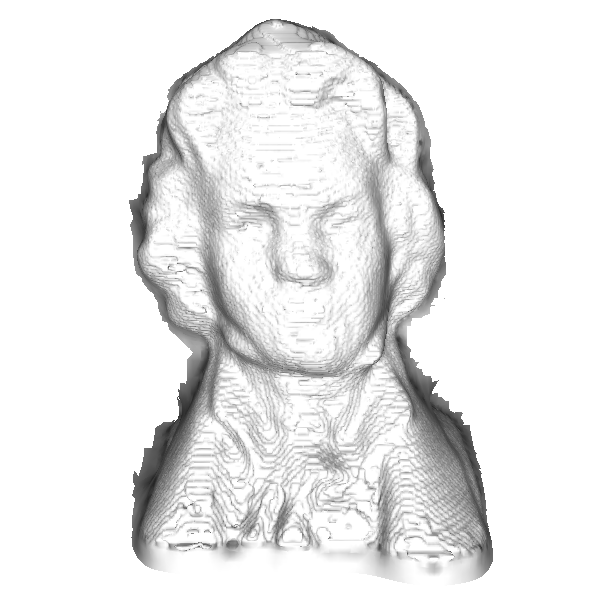
\includegraphics[width=0.1\textwidth]{interp/synth_interp/beethoven_sl}}&
\raisebox{-.5\height}{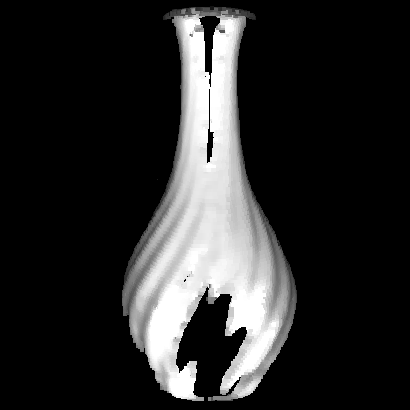
\includegraphics[width=0.1\textwidth]{interp/synth_interp/vase0_sl}}&
\fcolorbox{green}{white}{\raisebox{-.5\height}{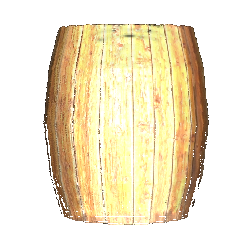
\includegraphics[width=0.1\textwidth]{interp/synth_interp/barrel_sl}}}&
\raisebox{-.5\height}{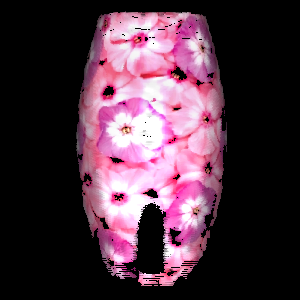
\includegraphics[width=0.1\textwidth]{interp/synth_interp/vase2_sl}}&
GSL\\
4 &
\raisebox{-.5\height}{\includegraphics[width=0.1\textwidth]{interp/synth_interp/beethoven_mvs}}&
\raisebox{-.5\height}{\includegraphics[width=0.1\textwidth]{interp/synth_interp/vase0_mvs}}&
\raisebox{-.5\height}{\includegraphics[width=0.1\textwidth]{interp/synth_interp/barrel_mvs}}&
\fcolorbox{green}{white}{\raisebox{-.5\height}{\includegraphics[width=0.1\textwidth]{interp/synth_interp/vase2_mvs}}}&
PMVS\\
\bottomrule
\end{tabular}
\end{figure}

\end{frame}

%------------------------------------------------
\begin{frame}{Interpretation: real-world objects}

\begin{figure}[!htbp]
\centering
\begin{tabular}{l|*{4}{p{1.5cm}}}
\toprule
prob cond\# & 1 & 2 & 3 & 4\\
\midrule
  & textureless & textureless & textured & textured\\
description & diffuse & mixed d/s & diffuse & mixed d/s\\
  & bright & bright & bright & bright\\
\hline
object & 
\raisebox{-.5\height}{\includegraphics[width=0.15\textwidth]{interp/real_world_img/statue/statue}} &
\raisebox{-.5\height}{\includegraphics[width=0.15\textwidth]{interp/real_world_img/cup/cup}} &
\raisebox{-.5\height}{\includegraphics[width=0.15\textwidth]{interp/real_world_img/pot/pot}} &
\raisebox{-.5\height}{\includegraphics[width=0.15\textwidth]{interp/real_world_img/vase/vase}}\\
\bottomrule
\end{tabular}
\caption{The rerepsentative real-world objects of the four problem conditions for evaluation.}
\end{figure}

\end{frame}

%------------------------------------------------
\begin{frame}{Interpretation: evaluation of interpreter (cont'd)}

\begin{figure}[!htbp]
\centering
\begin{tabular}{lccccr}
\toprule
Desc \# & Statue & Cup & Pot & Vase & Interp Algo.\\
\midrule
1 &
\fcolorbox{green}{white}{\raisebox{-.5\height}{\includegraphics[width=0.1\textwidth]{interp/real_interp/statue/statue_sl}}}&
\raisebox{-.5\height}{\includegraphics[width=0.1\textwidth]{interp/real_interp/cup/cup_sl}}&
\raisebox{-.5\height}{\includegraphics[width=0.1\textwidth]{interp/real_interp/pot/pot_sl}}&
\raisebox{-.5\height}{\includegraphics[width=0.1\textwidth]{interp/real_interp/vase/vase_sl}}&
GSL\\
2 &
\raisebox{-.5\height}{\includegraphics[width=0.1\textwidth]{interp/real_interp/statue/statue_ps}}&
\fcolorbox{green}{white}{\raisebox{-.5\height}{\includegraphics[width=0.1\textwidth]{interp/real_interp/cup/cup_ps}}}&
\raisebox{-.5\height}{\includegraphics[width=0.1\textwidth]{interp/real_interp/pot/pot_ps}}&
\raisebox{-.5\height}{\includegraphics[width=0.1\textwidth]{interp/real_interp/vase/vase_ps}}&
EPS\\
3 &
\raisebox{-.5\height}{\includegraphics[width=0.1\textwidth]{interp/real_interp/statue/statue_sl}}&
\raisebox{-.5\height}{\includegraphics[width=0.1\textwidth]{interp/real_interp/cup/cup_sl}}&
\fcolorbox{green}{white}{\raisebox{-.5\height}{\includegraphics[width=0.1\textwidth]{interp/real_interp/pot/pot_sl}}}&
\raisebox{-.5\height}{\includegraphics[width=0.1\textwidth]{interp/real_interp/vase/vase_sl}}&
GSL\\
4 &
\raisebox{-.5\height}{\includegraphics[width=0.1\textwidth]{interp/real_interp/statue/statue_mvs}}&
\raisebox{-.5\height}{\includegraphics[width=0.1\textwidth]{interp/real_interp/cup/cup_mvs}}&
\raisebox{-.5\height}{\includegraphics[width=0.1\textwidth]{interp/real_interp/pot/pot_mvs}}&
\fcolorbox{green}{white}{\raisebox{-.5\height}{\includegraphics[width=0.1\textwidth]{interp/real_interp/vase/vase_mvs}}}&
PMVS\\
\bottomrule
\end{tabular}
\end{figure}

\end{frame}

%------------------------------------------------
\begin{frame}{Interpretation: discussion}

\end{frame}

%------------------------------------------------
\section{Conclusions}
%------------------------------------------------
\begin{frame}{Conclusions}

\begin{itemize}
\item the proposed description is able to give correct reconstruction for non-concave objects
\item To deal with more complicated objects, we need more complicated properties, or ways to describe the objects, but the challenge is the easy mathematical representation might not be available.
\item Using the simple descriptive language and proof-of-concept interpreter, we demonstrate the possibility of using descriptive properties to hide algorithmic details.
\end{itemize}
\end{frame}

%------------------------------------------------
\begin{frame}[standout]{Take-away message}

Computer vision should focus on more than \\just algorithms, but easier accessibility.

\end{frame}

\end{document}
